\documentclass[hyperref,UTF8]{ctexart}
\usepackage[dvipdfmx]{graphicx}
\usepackage{gbt7714}
\usepackage{float}
\usepackage{ragged2e}
\usepackage{amsthm}
\usepackage{amssymb}
\usepackage{amsmath}
\usepackage{wrapfig}
\usepackage{tikz}
\usetikzlibrary{arrows.meta}
\usepackage{booktabs}
\usepackage[a4paper,left=3.18cm,right=3.18cm,top=2.54cm,bottom=2.54cm]{geometry}
\usepackage{tabularx}
\usepackage{array}
\usepackage{caption}
\usepackage{hyperref}
\newcommand{\upcite}[1]{\textsuperscript{\textsuperscript{\cite{#1}}}}
\setCJKfamilyfont{song}{SimSun}
\title{Self-Introduction \& Plan}
\author{赵翔}
\begin{document}
\maketitle
\part{自我介绍}
\section{高中及之前的环境}
我来自内蒙古呼和浩特,是一座美丽的城市
\begin{figure}[H]
    \centering
    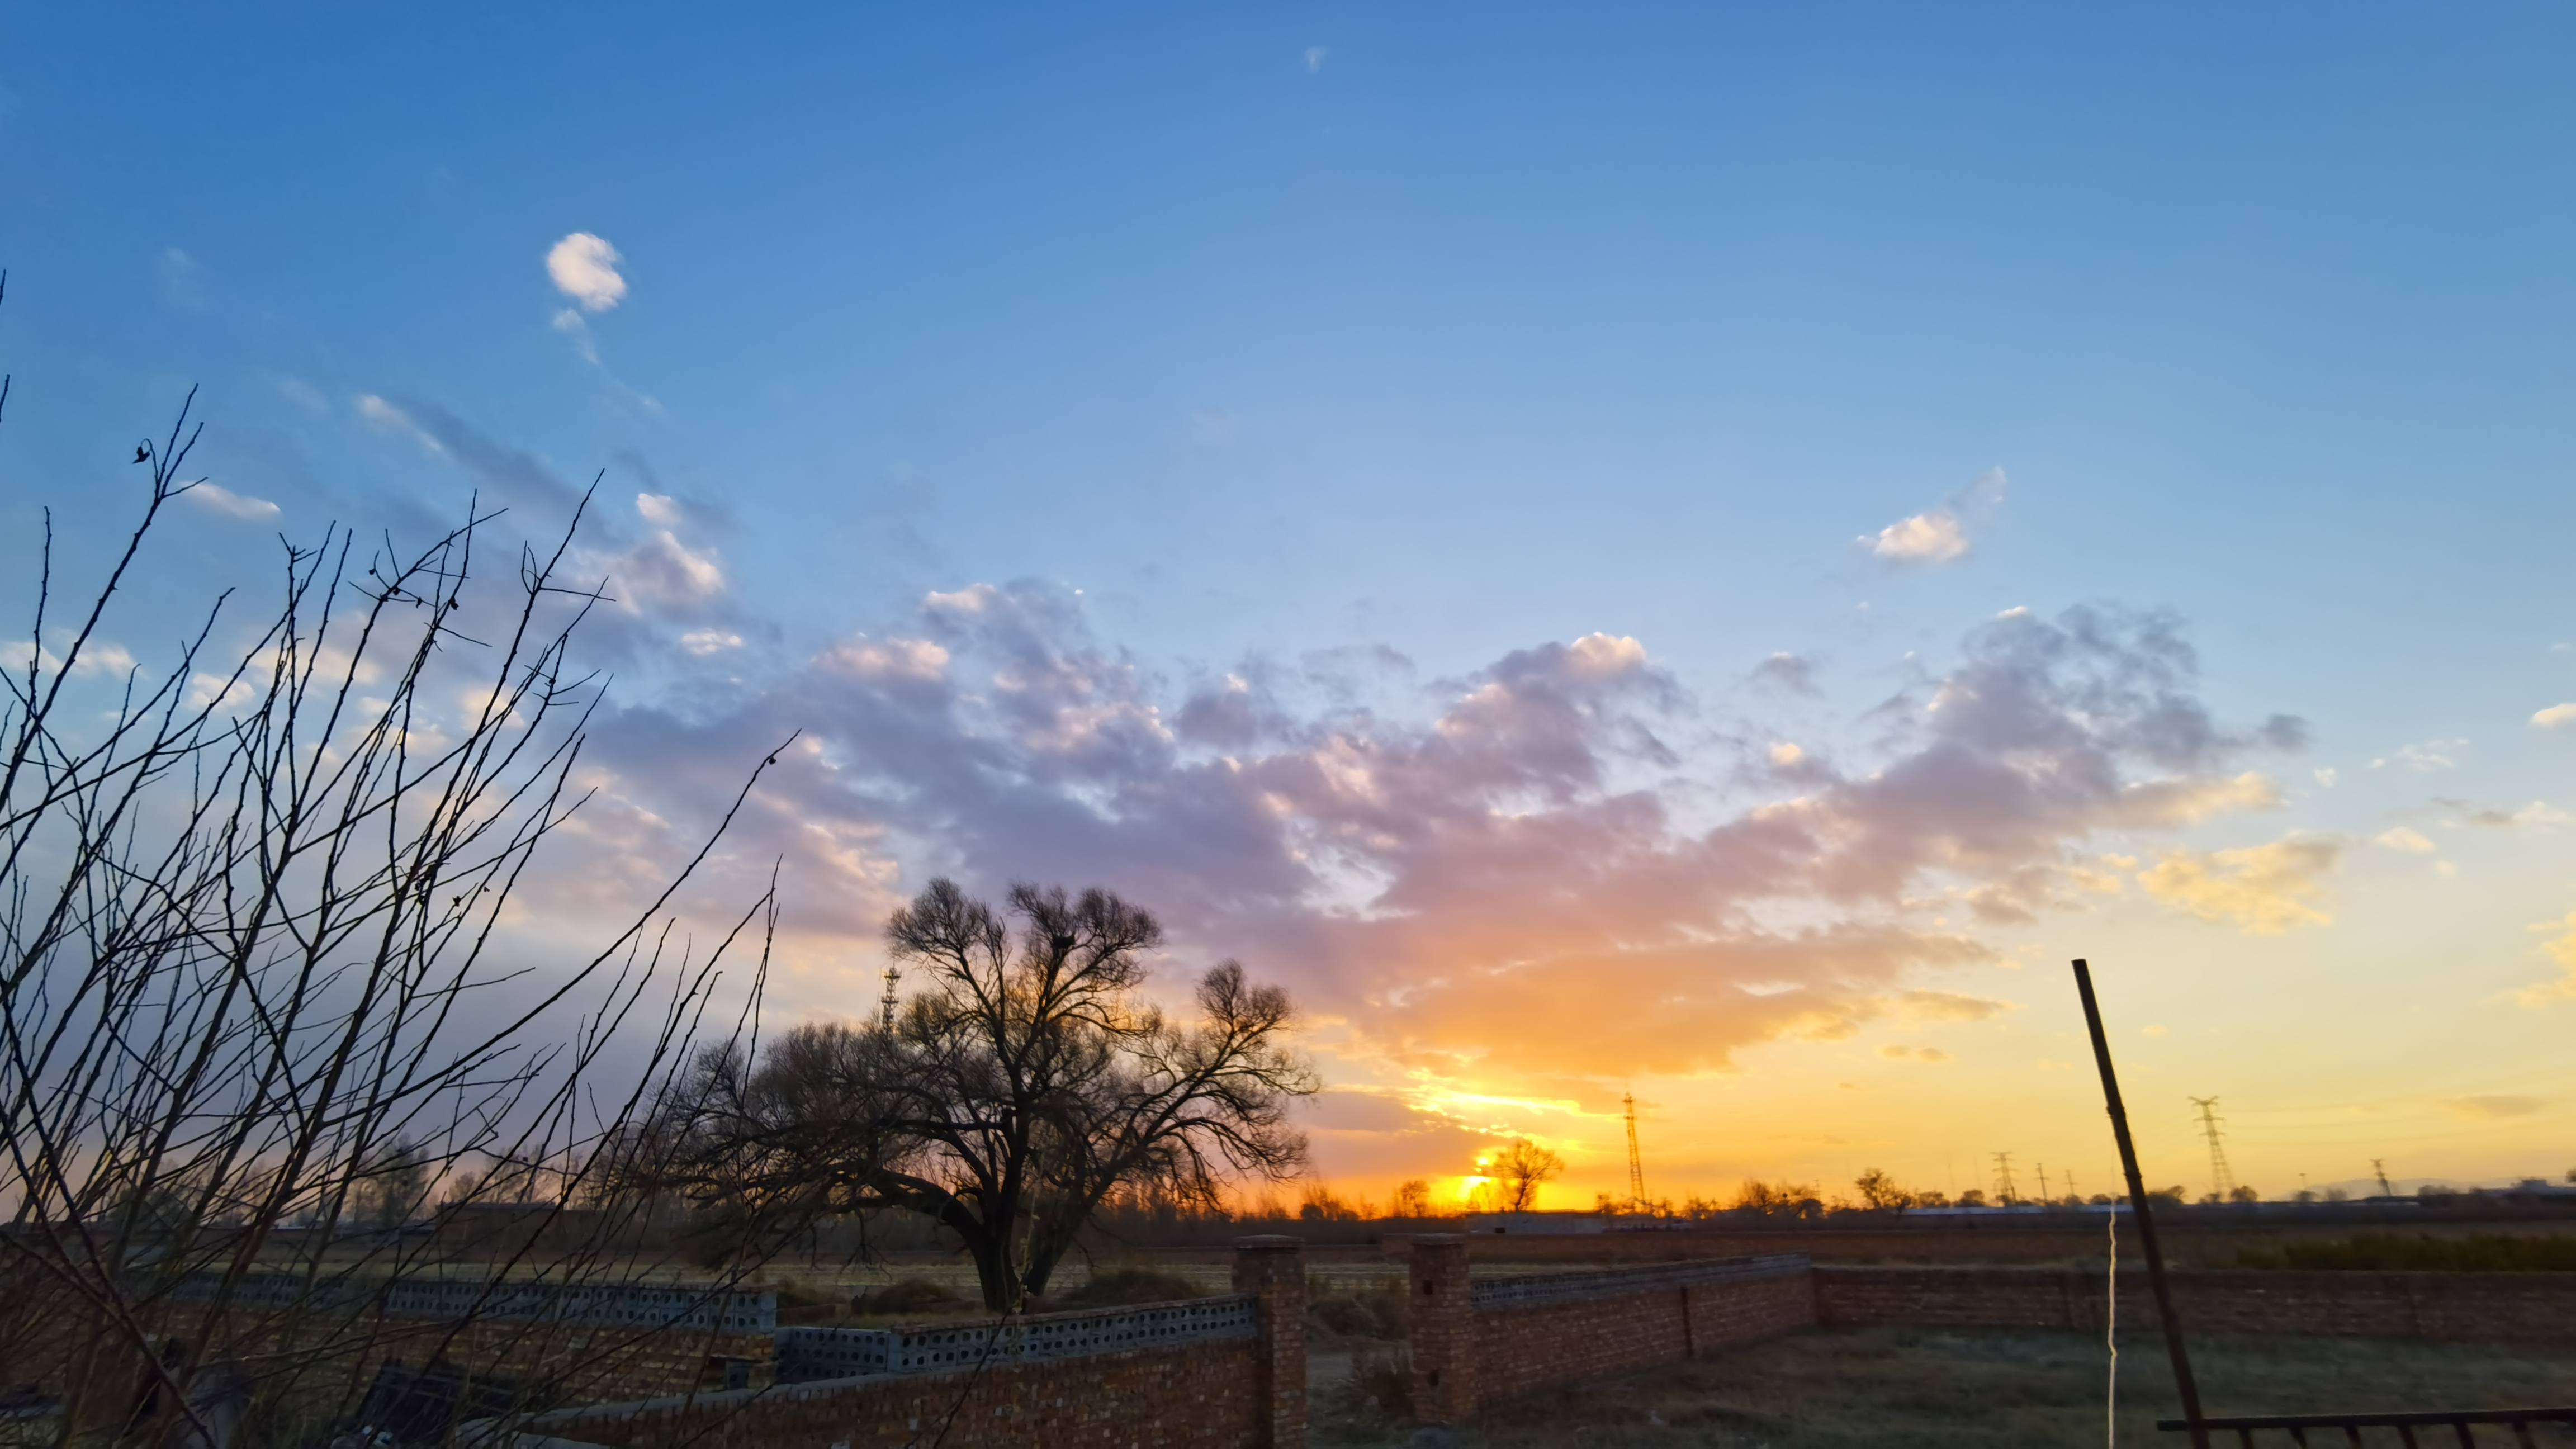
\includegraphics[width=8cm]{IMG_20210206_174128.jpg}
\end{figure}
高中毕业于呼和浩特市第二中学,这所高中由爱国名将傅作义创立于1942年,所以山西大学120周年校庆时,也会迎来高中母校的80年华诞。
\begin{figure}[H]
    \centering
    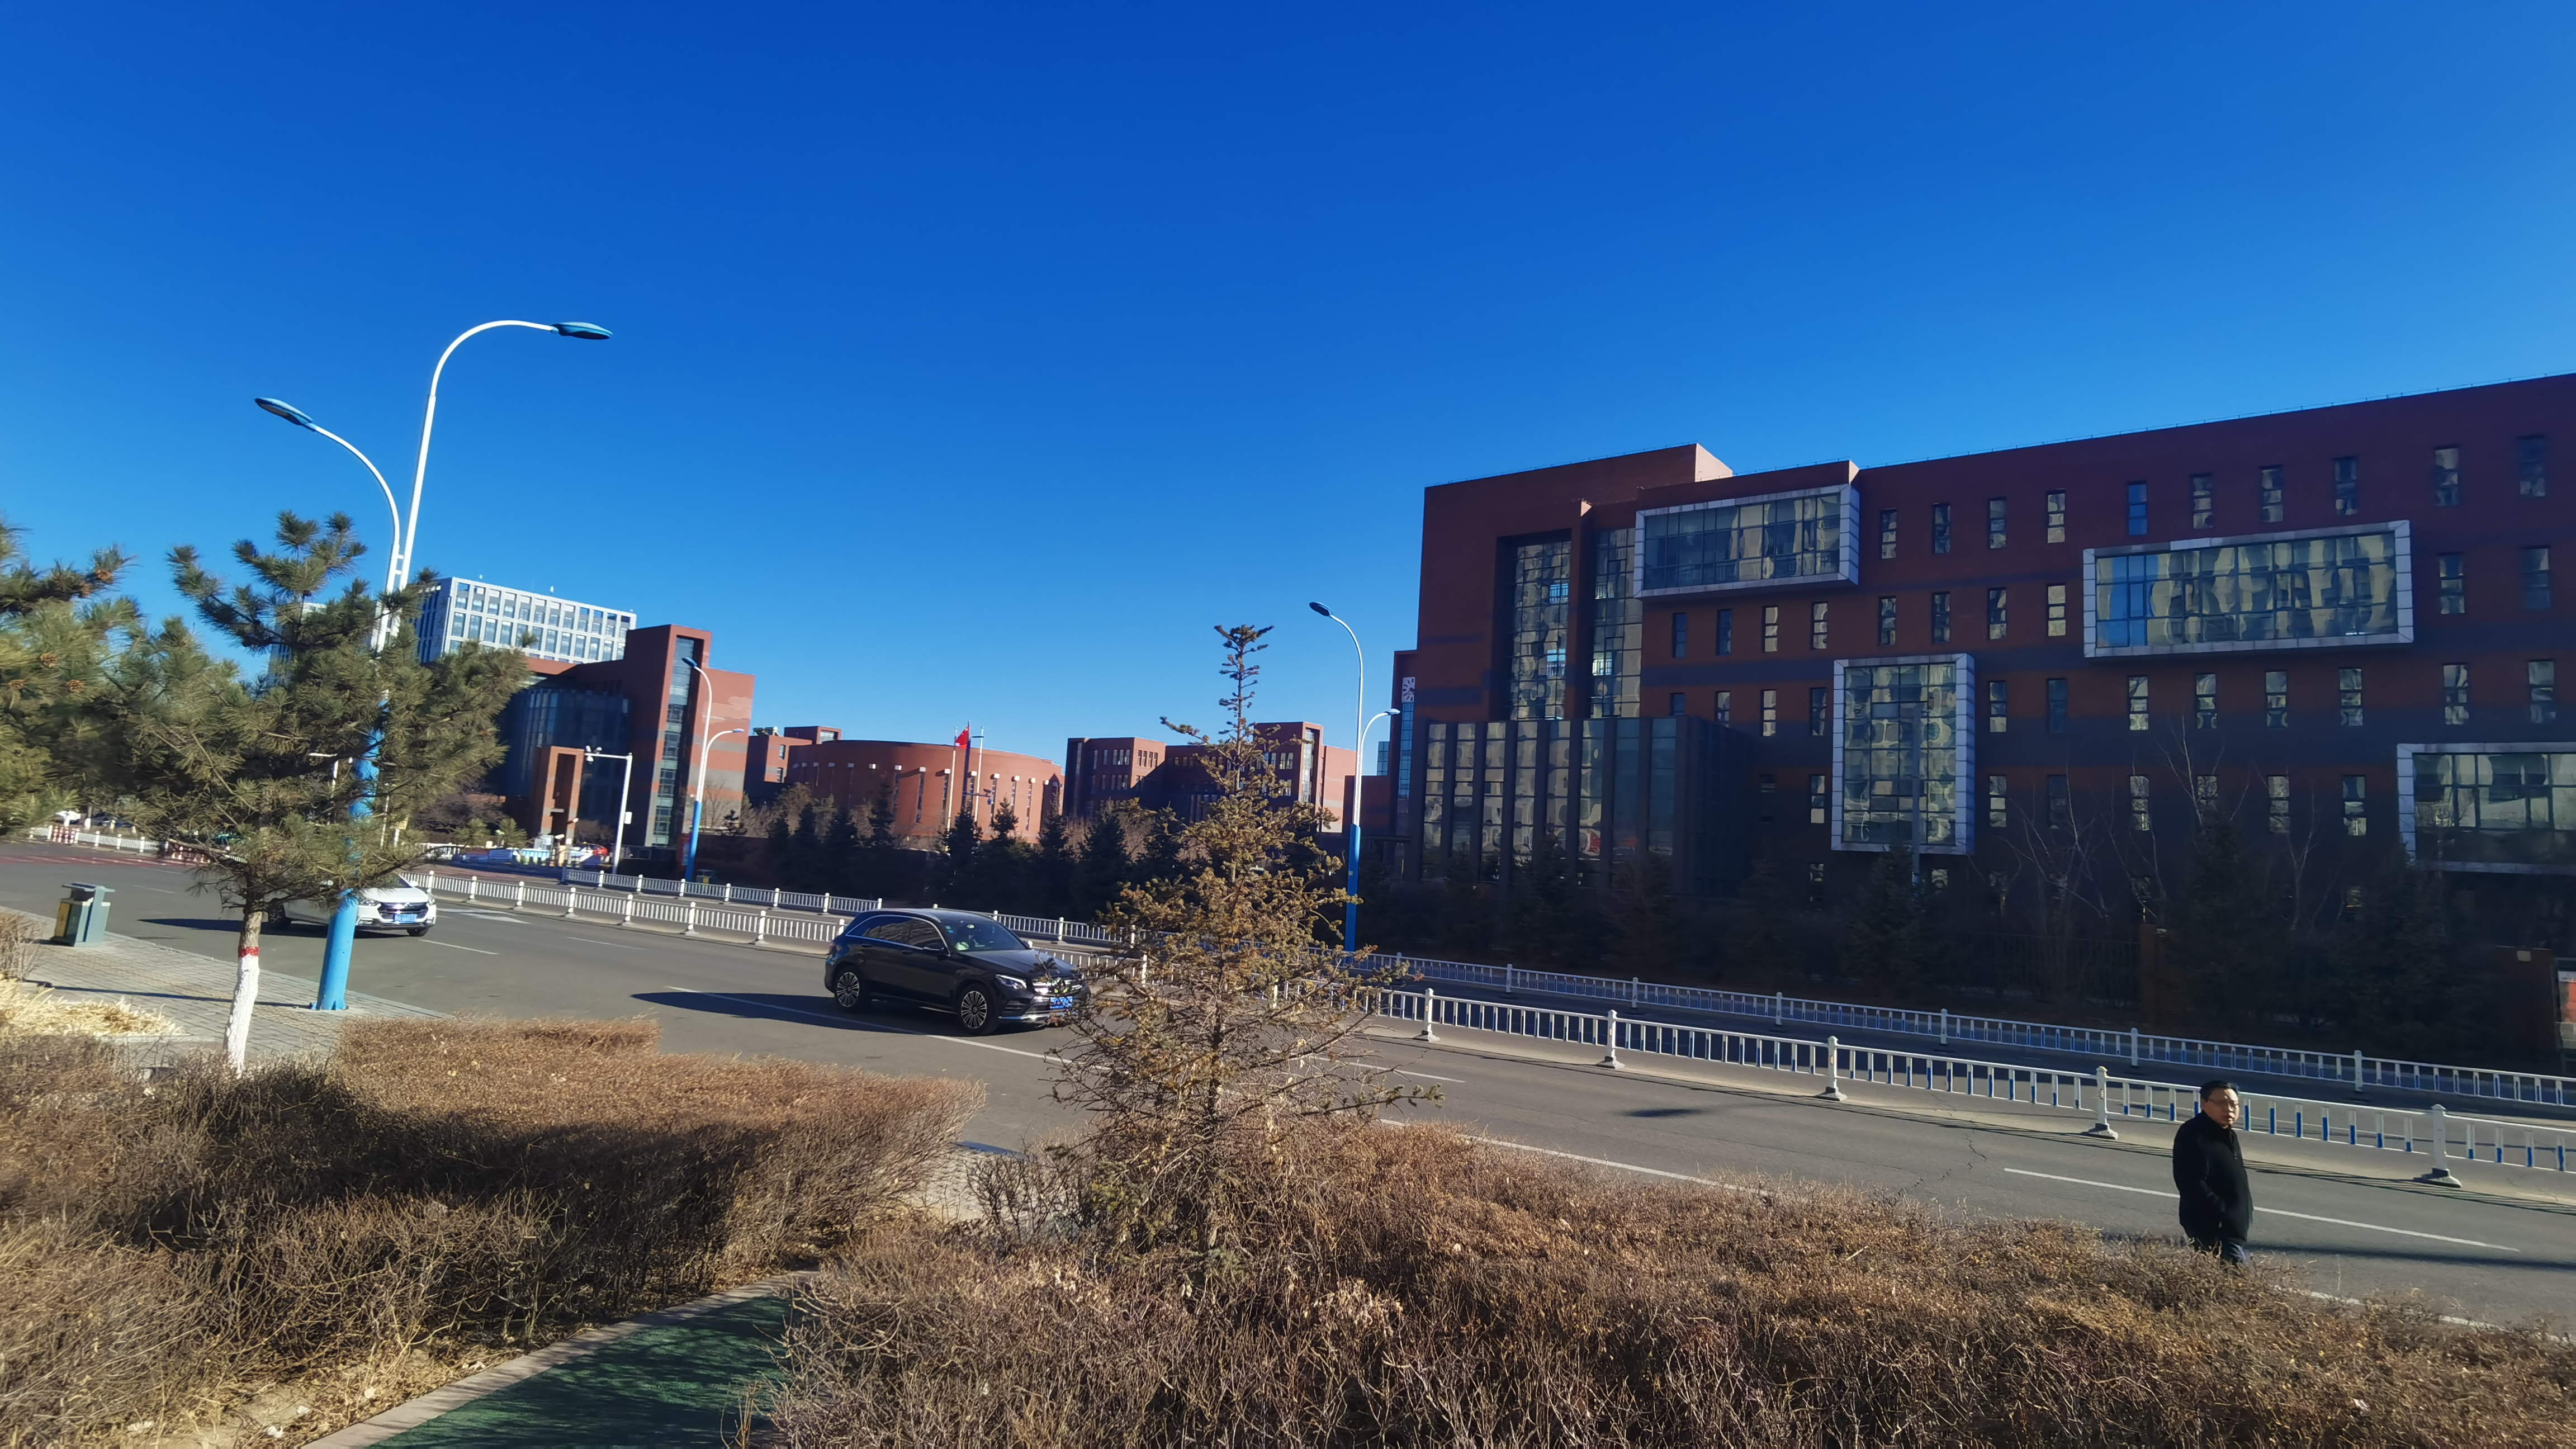
\includegraphics[width=8cm]{IMG_20210207_152437.jpg}
\end{figure}
其实呼和浩特或是内蒙古并不是人们印象中的遍地草原,而也是现代化的都市,和太原其实相差不大。呼和浩特第二中学也是内蒙古综合实力最强的一所高中。
\section{高中及之前的我自己}
从初中开始,我便逐渐对数学物理感兴趣,未来能在高中学习物理竞赛,初中我便自学高等数学,当时用的是同济的第5版,这本书中规中矩,也比较适合入门,然而我当时的理解能力比较差,一些基本的概念往往要好几天才能想明白,但是想明白了之后就会很开心,就是这样的兴奋感和对新知识的渴求,当我步入高中的时候,也延续了这样的做法,我开始学习普通物理,使用的是赵凯华的一套《新概念物理学》,这套书很好也很有难度,我直到现在也不算是“学通”了这套书,尤其是后面的光学热学近代物理,把很多四大力学的东西下放,更加强了它的难度。配合当时竞赛的必读书目“程书”,开始了我的竞赛经历。
\begin{figure}[H]
    \centering
    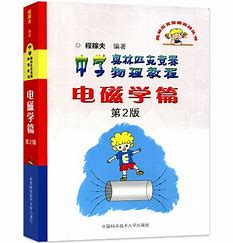
\includegraphics[width=4cm]{程书.jpg}
    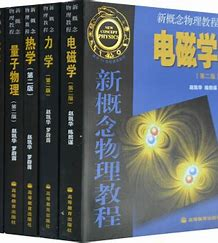
\includegraphics[width=4cm]{新概念.jpg}
\end{figure}
内蒙古是所谓的“竞赛弱省”,竞赛资源少的离谱,所以我只能在其他省寻求资源,找全国性的竞赛教育机构组织的夏令营和冬令营,这些培训的机会让我走遍全国各地,见识各种各样的其他省的学生,让我深刻感受到了地域之间的教育资源的差距,也让我有幸能接触到中国最年轻的一批优秀的物理学习者,这让我在高中就完成了要在大学完成的开阔视野的工作,也学完了大部分的竞赛要求的物理知识。高二参加了第35届全国中学生物理竞赛,因为实验的差错与省一等奖擦肩而过。
\begin{figure}[H]
    \centering
    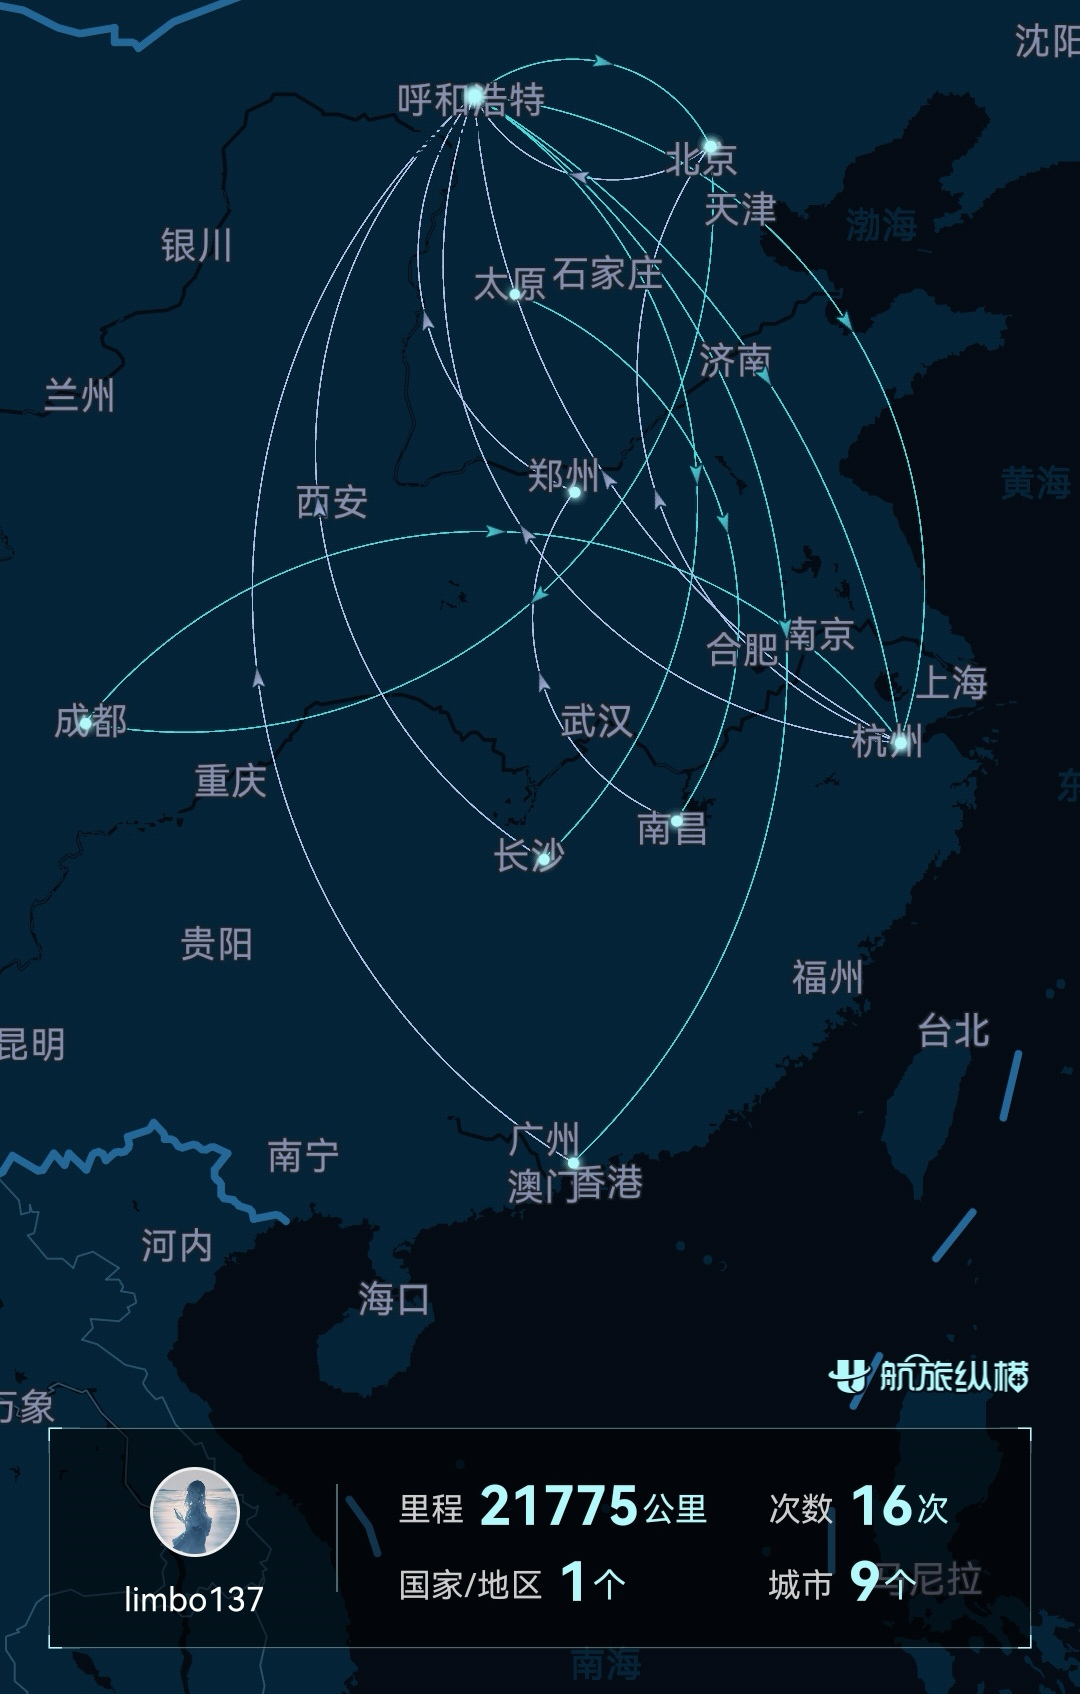
\includegraphics[width=4.2cm]{Screenshot_20210907_104729_com.umetrip.android.msky.app_edit_578928791734057.jpg}
    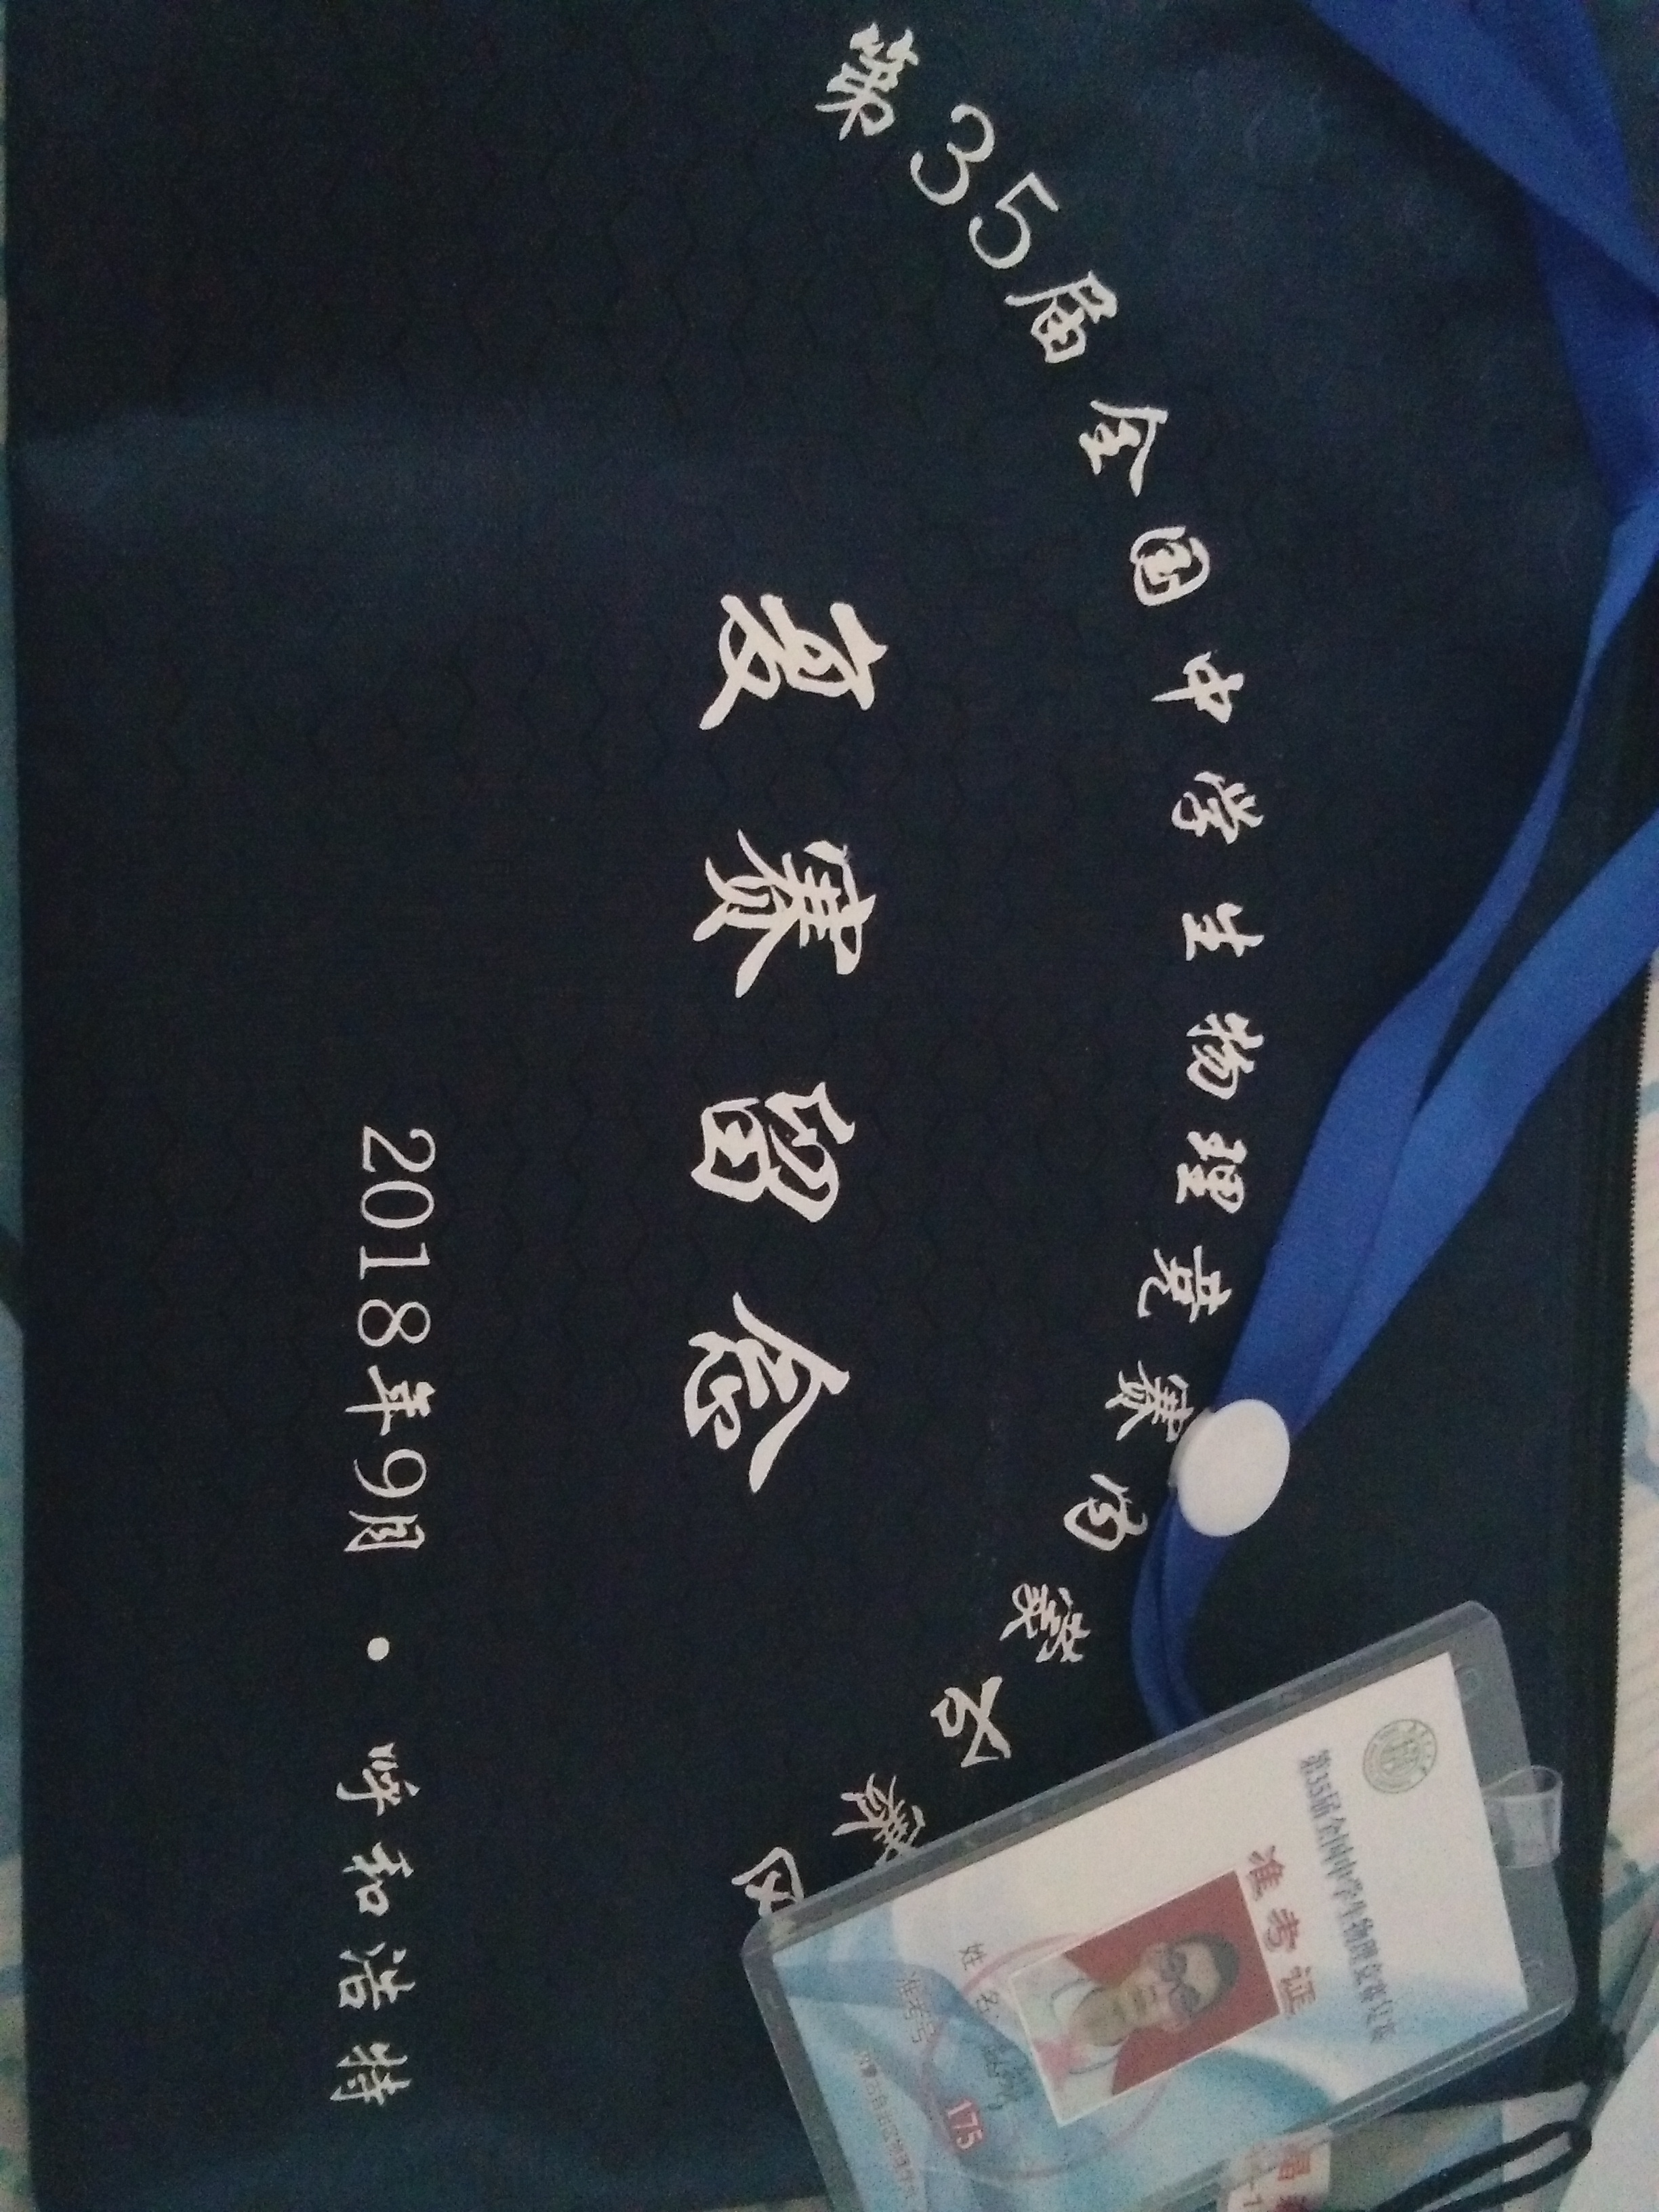
\includegraphics[width=5cm]{IMG_20180922_072940.jpg}
\end{figure}
那年的理论题目很新颖,我比较喜欢,当时的简谐振动的题目结合了相图,还有一个螺纹干涉的光学题目,但确实很考验思维量。
\begin{figure}[H]
    \centering
    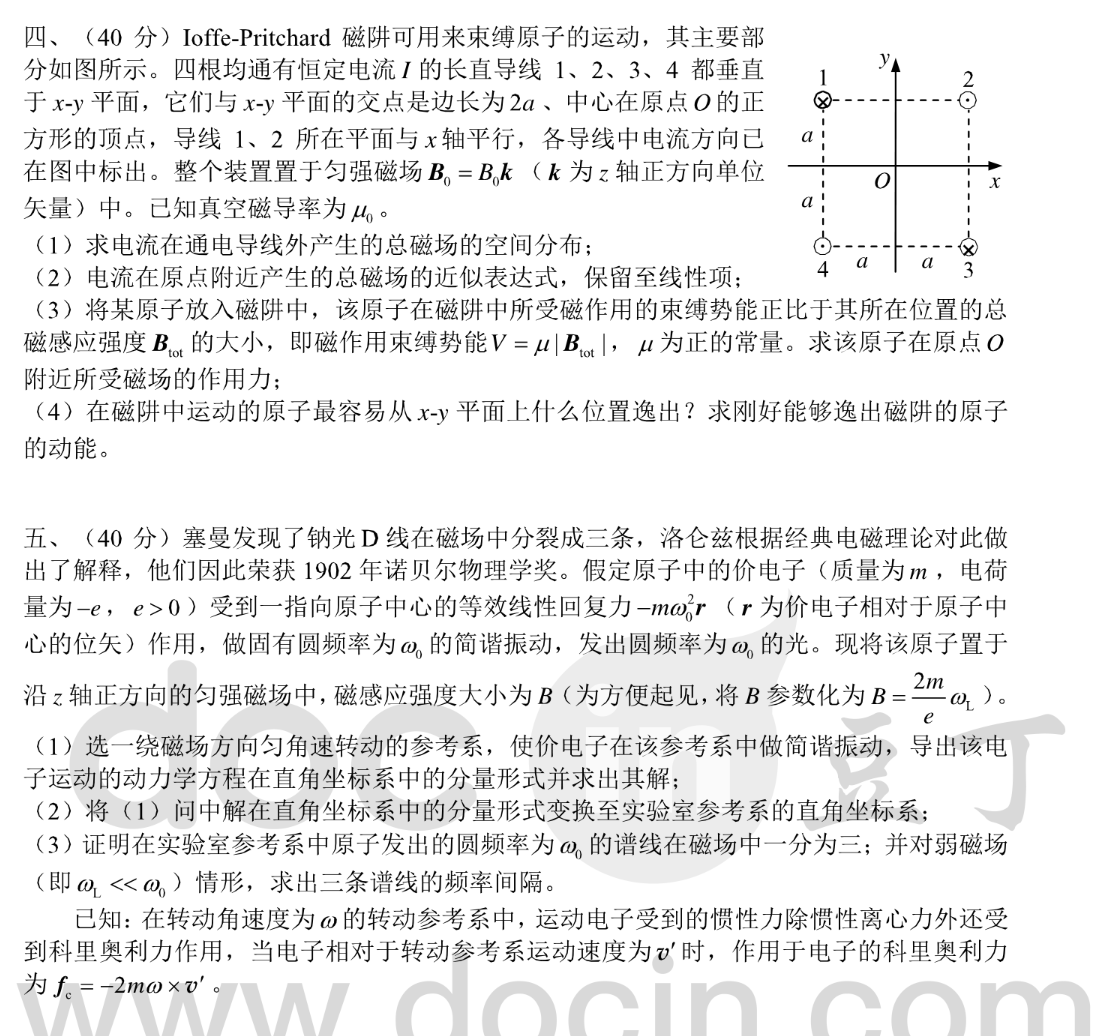
\includegraphics[width=6cm]{屏幕截图 2021-09-07 110713.png}
    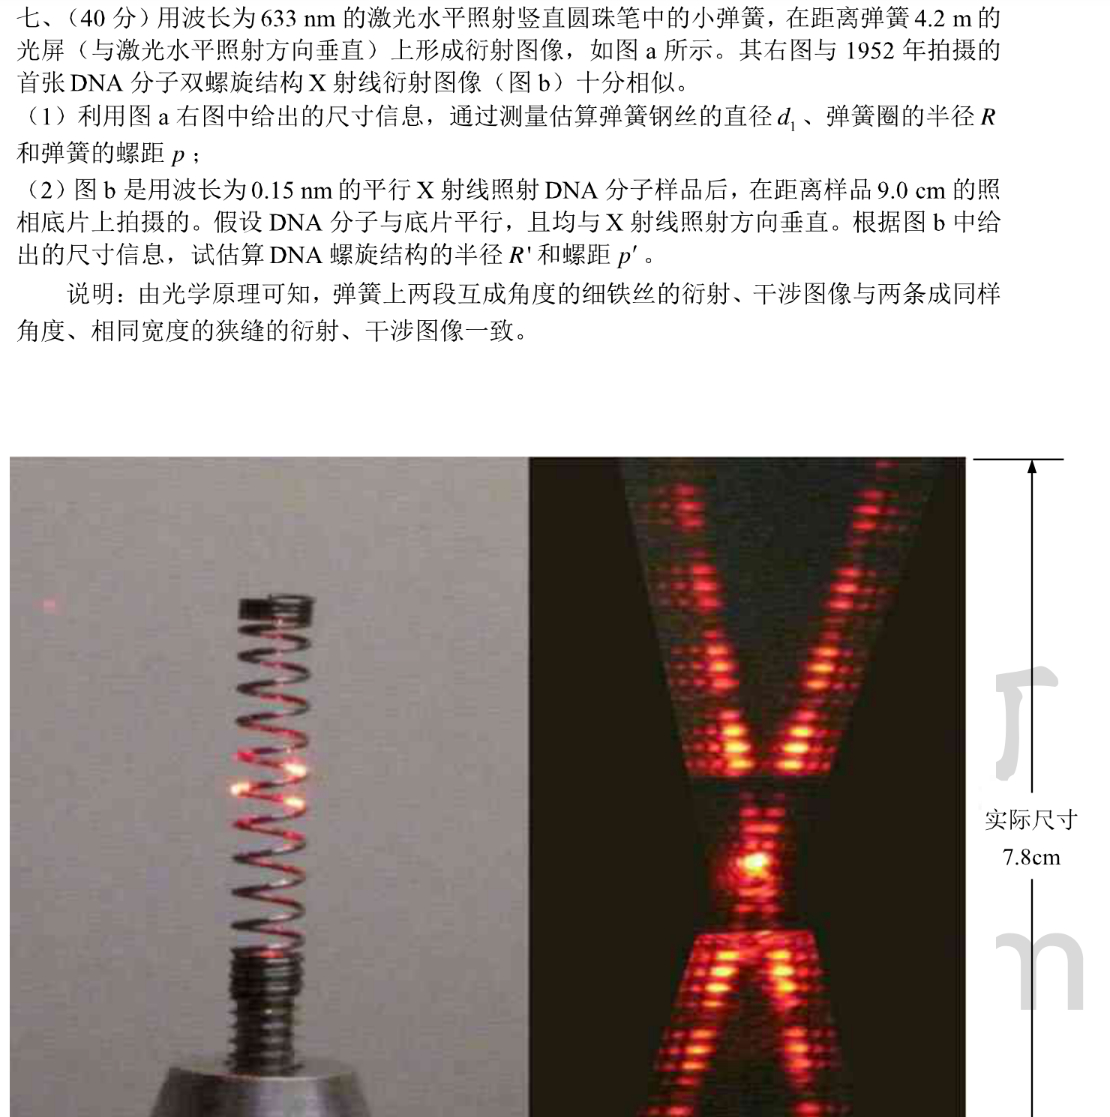
\includegraphics[width=6cm]{屏幕截图 2021-09-07 110937.png}
\end{figure}
高二我便开始潜心反思和总结,还有继续从前的学习,主要便是舒幼生老先生的《题选》,还有对程书的细节的把握,第一次考试的失败让我逐渐反思我应该做什么,在高二下半年,我开始停课.
\begin{figure}[H]
    \centering
    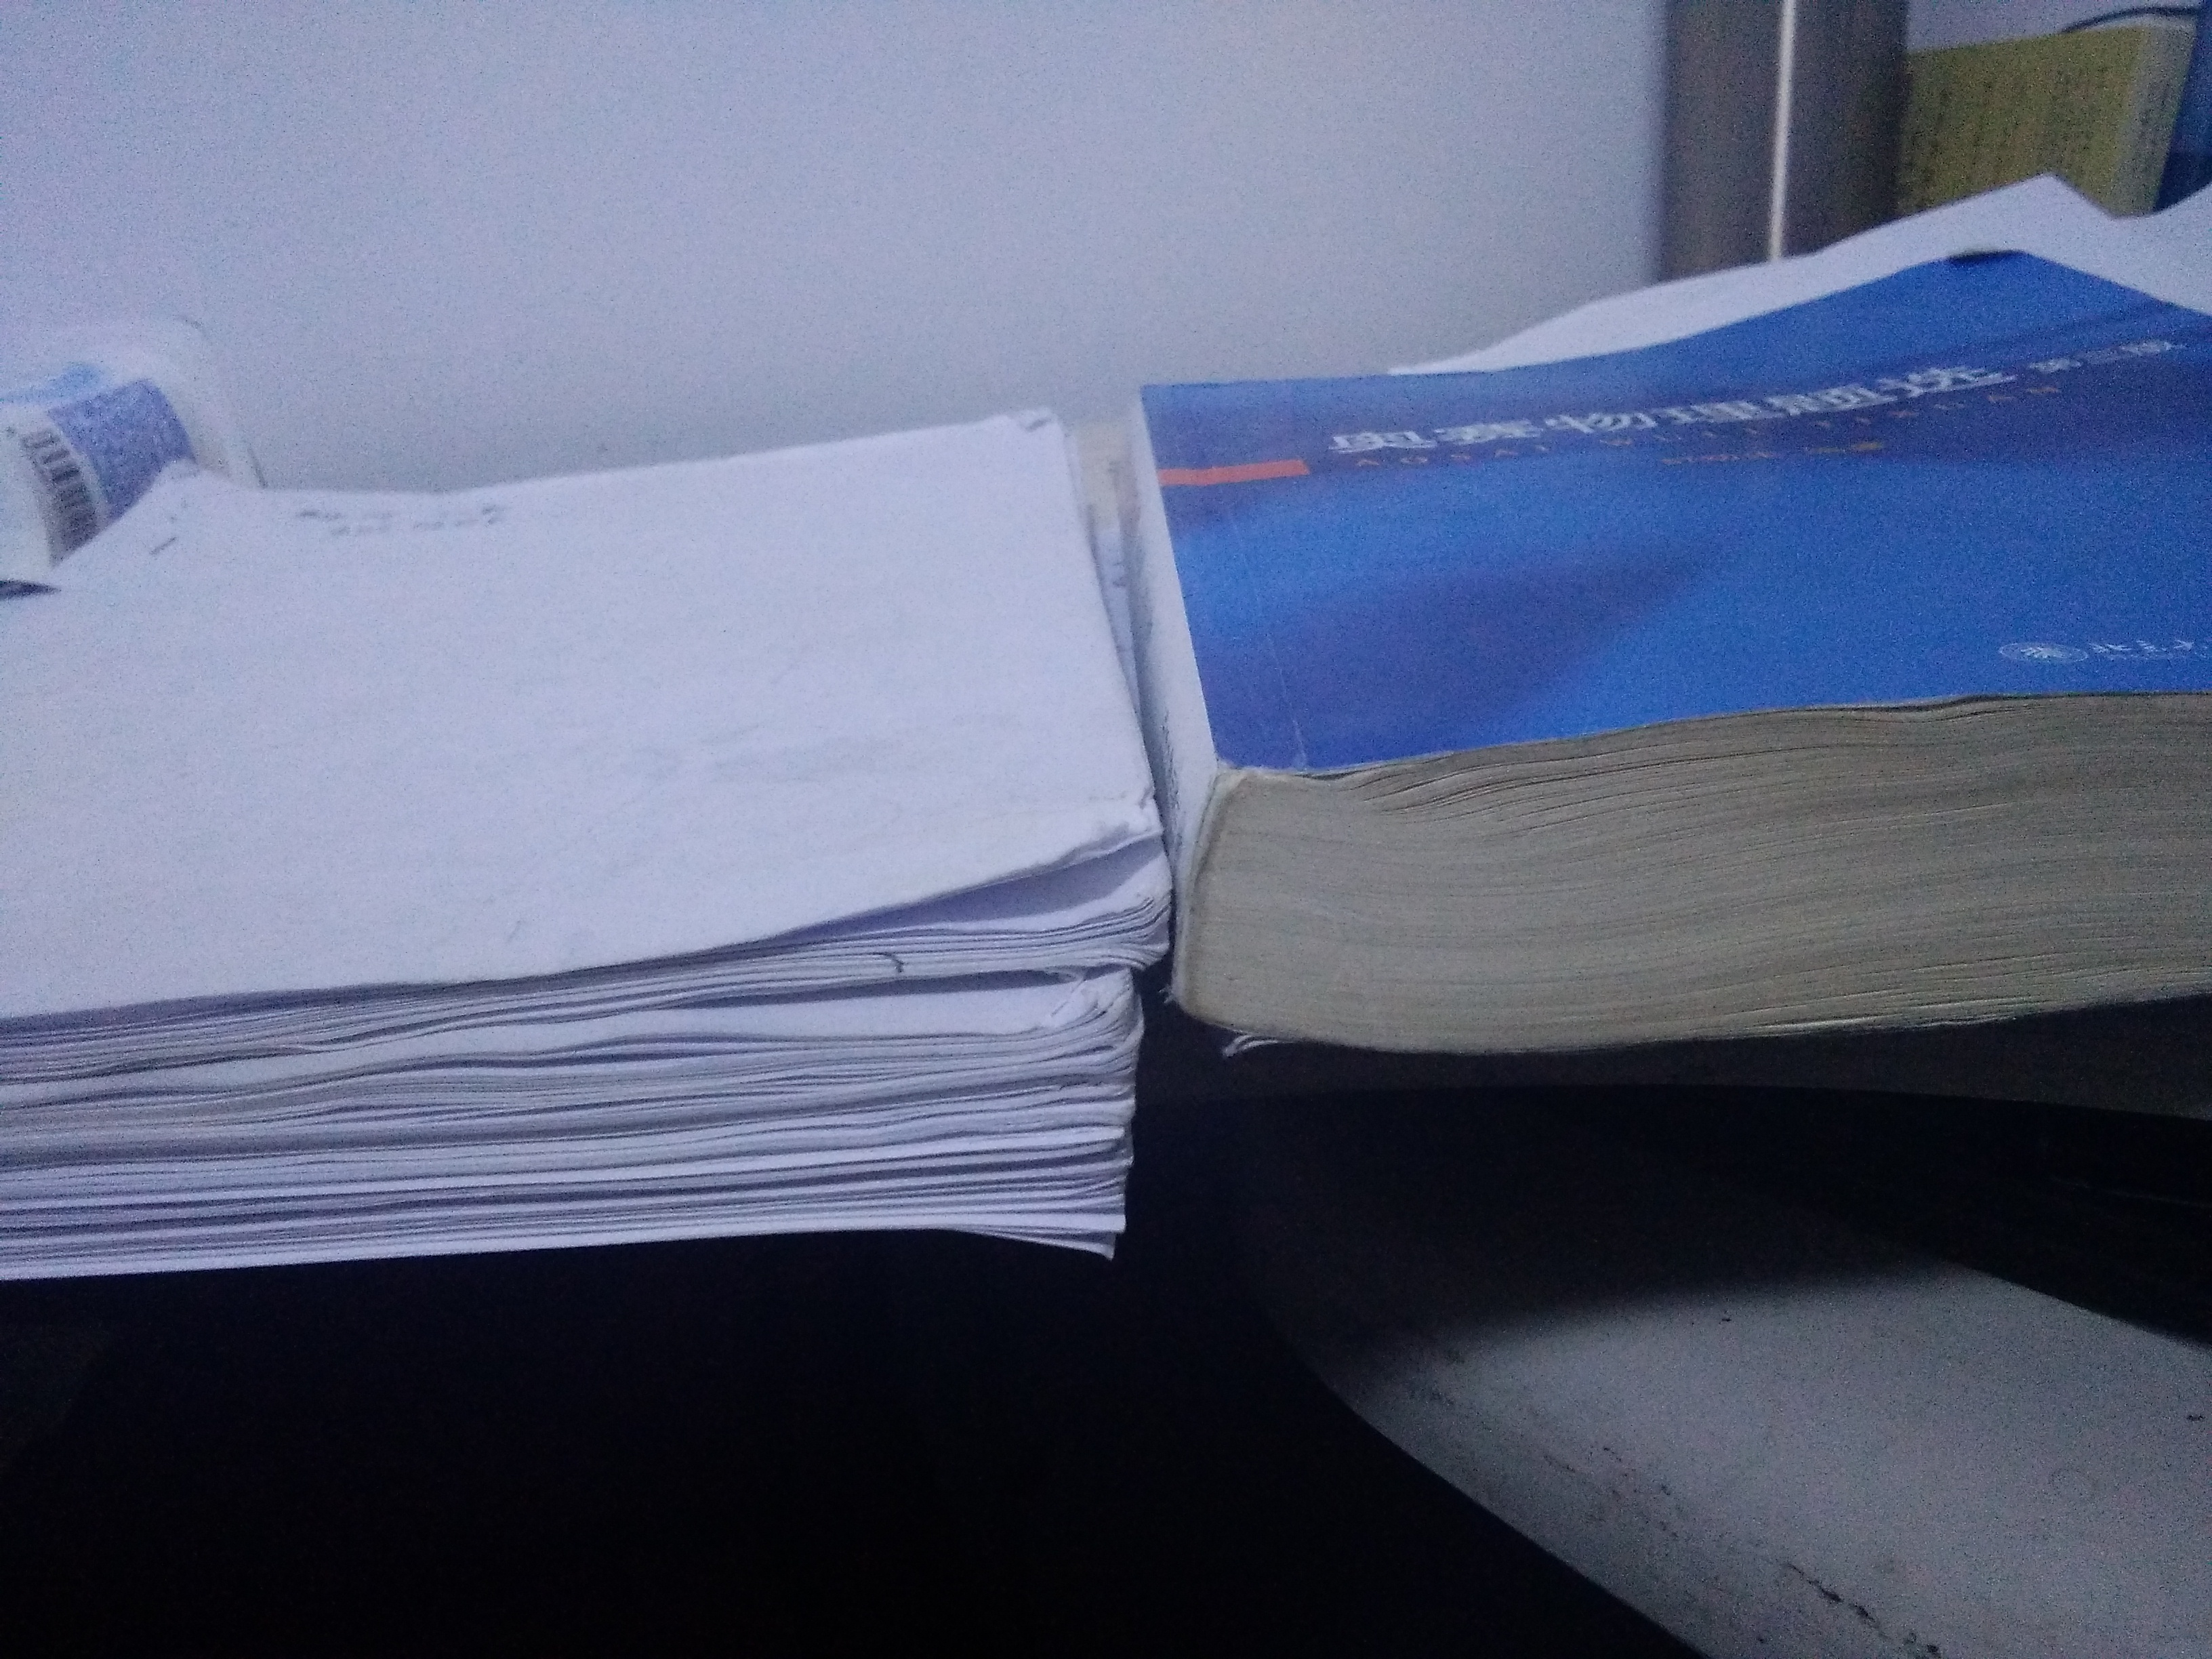
\includegraphics[width=6cm]{IMG_20190425_003812.jpg}
    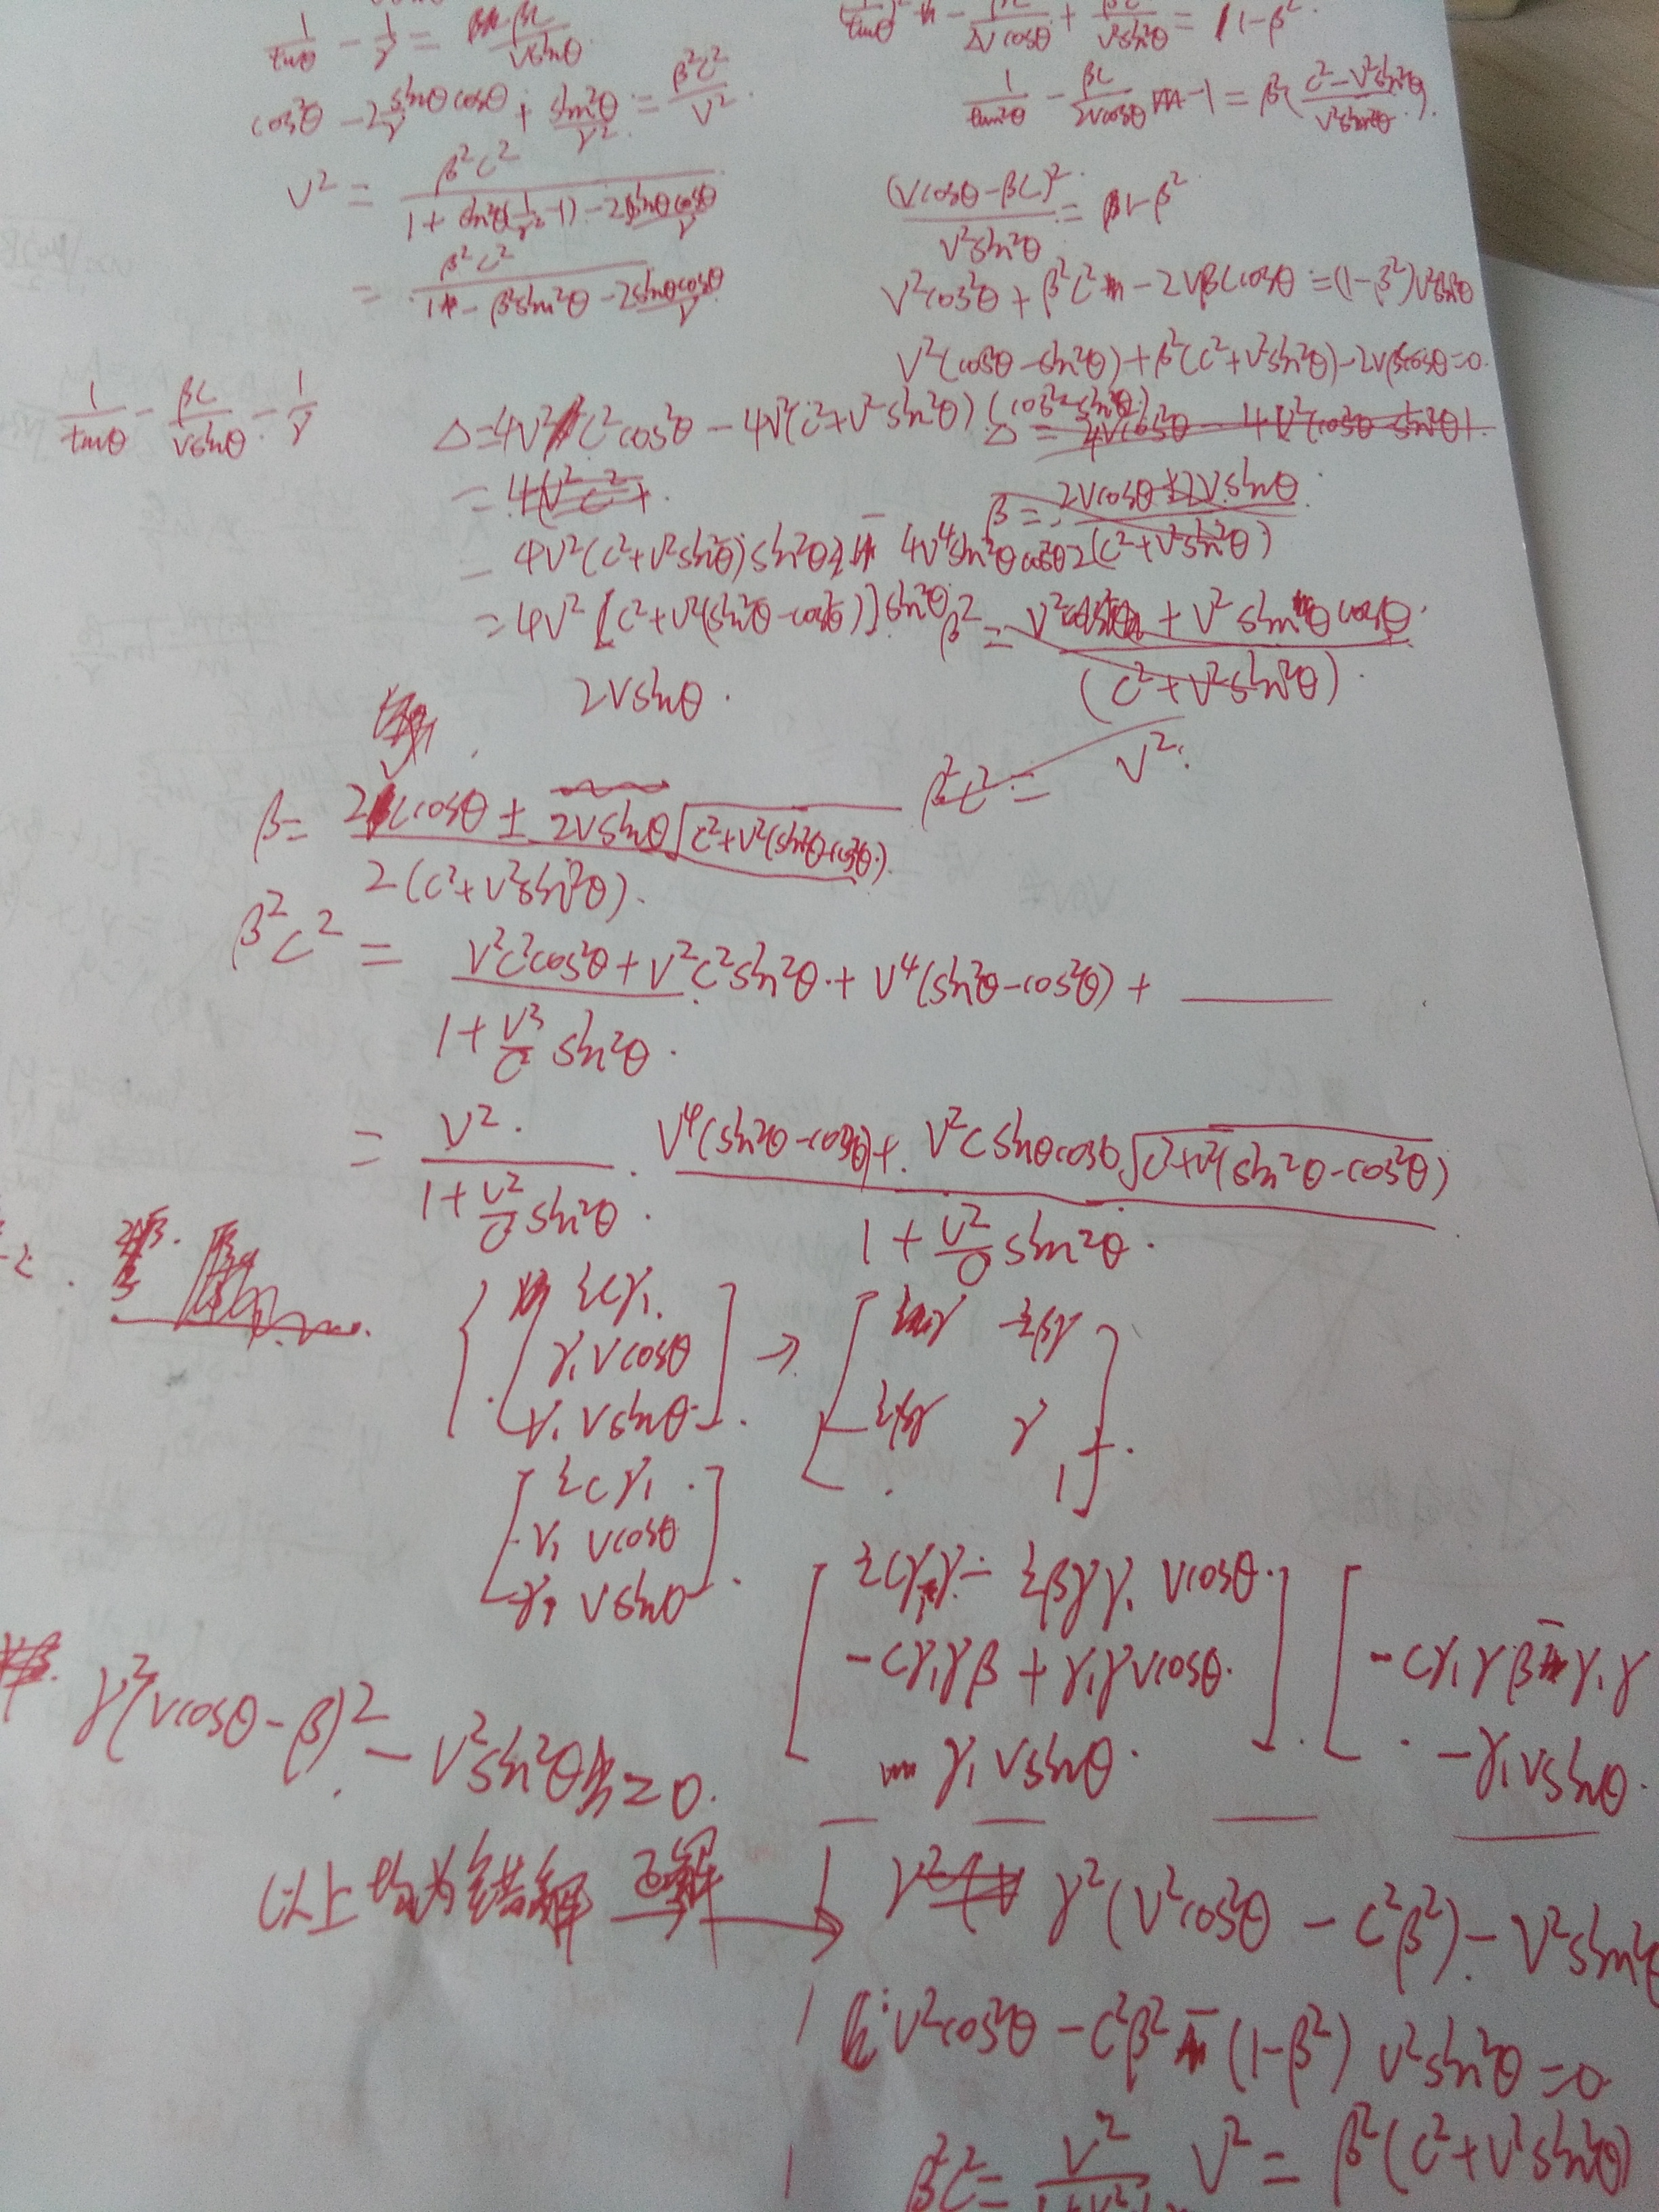
\includegraphics[width=4cm]{IMG_20190530_080259.jpg}
    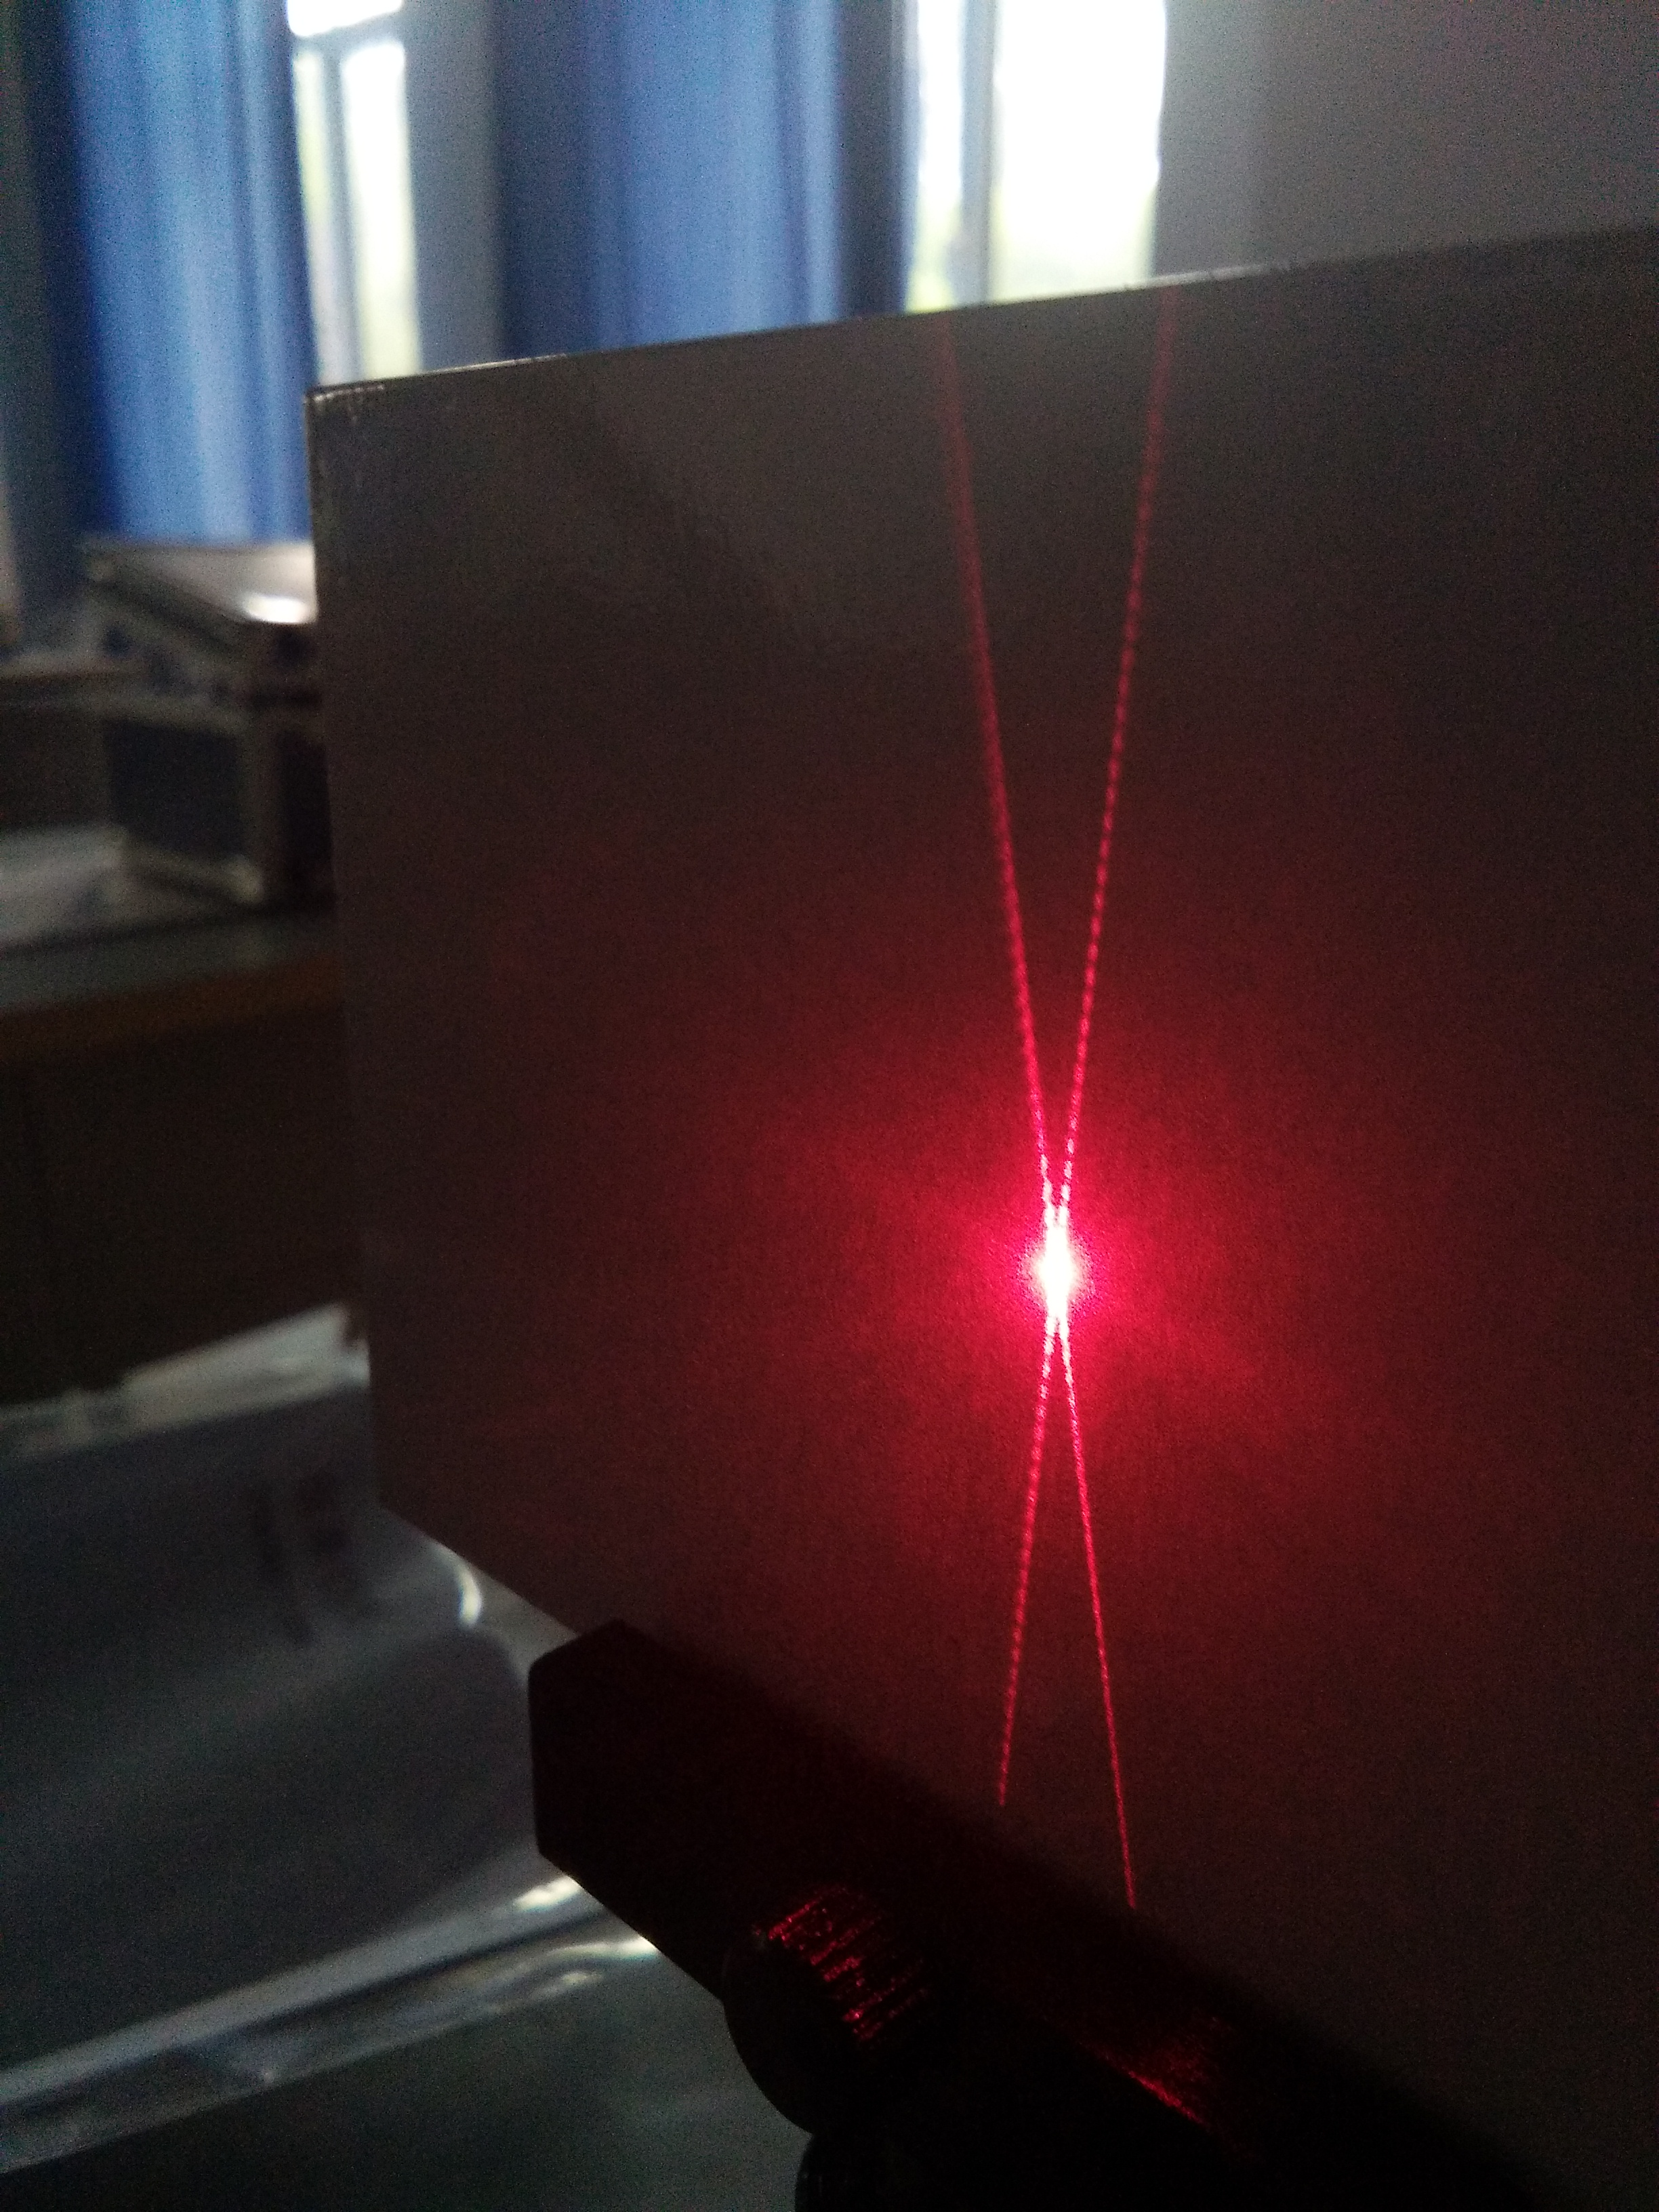
\includegraphics[width=4cm]{IMG_20190529_184626.jpg}
\end{figure}
那段一个人的时间在后面比较难熬,不过也让我潜下心来,那时恰逢春夏之交,有点“春风化雨,细推物理”的感觉了
\begin{figure}[H]
    \centering
    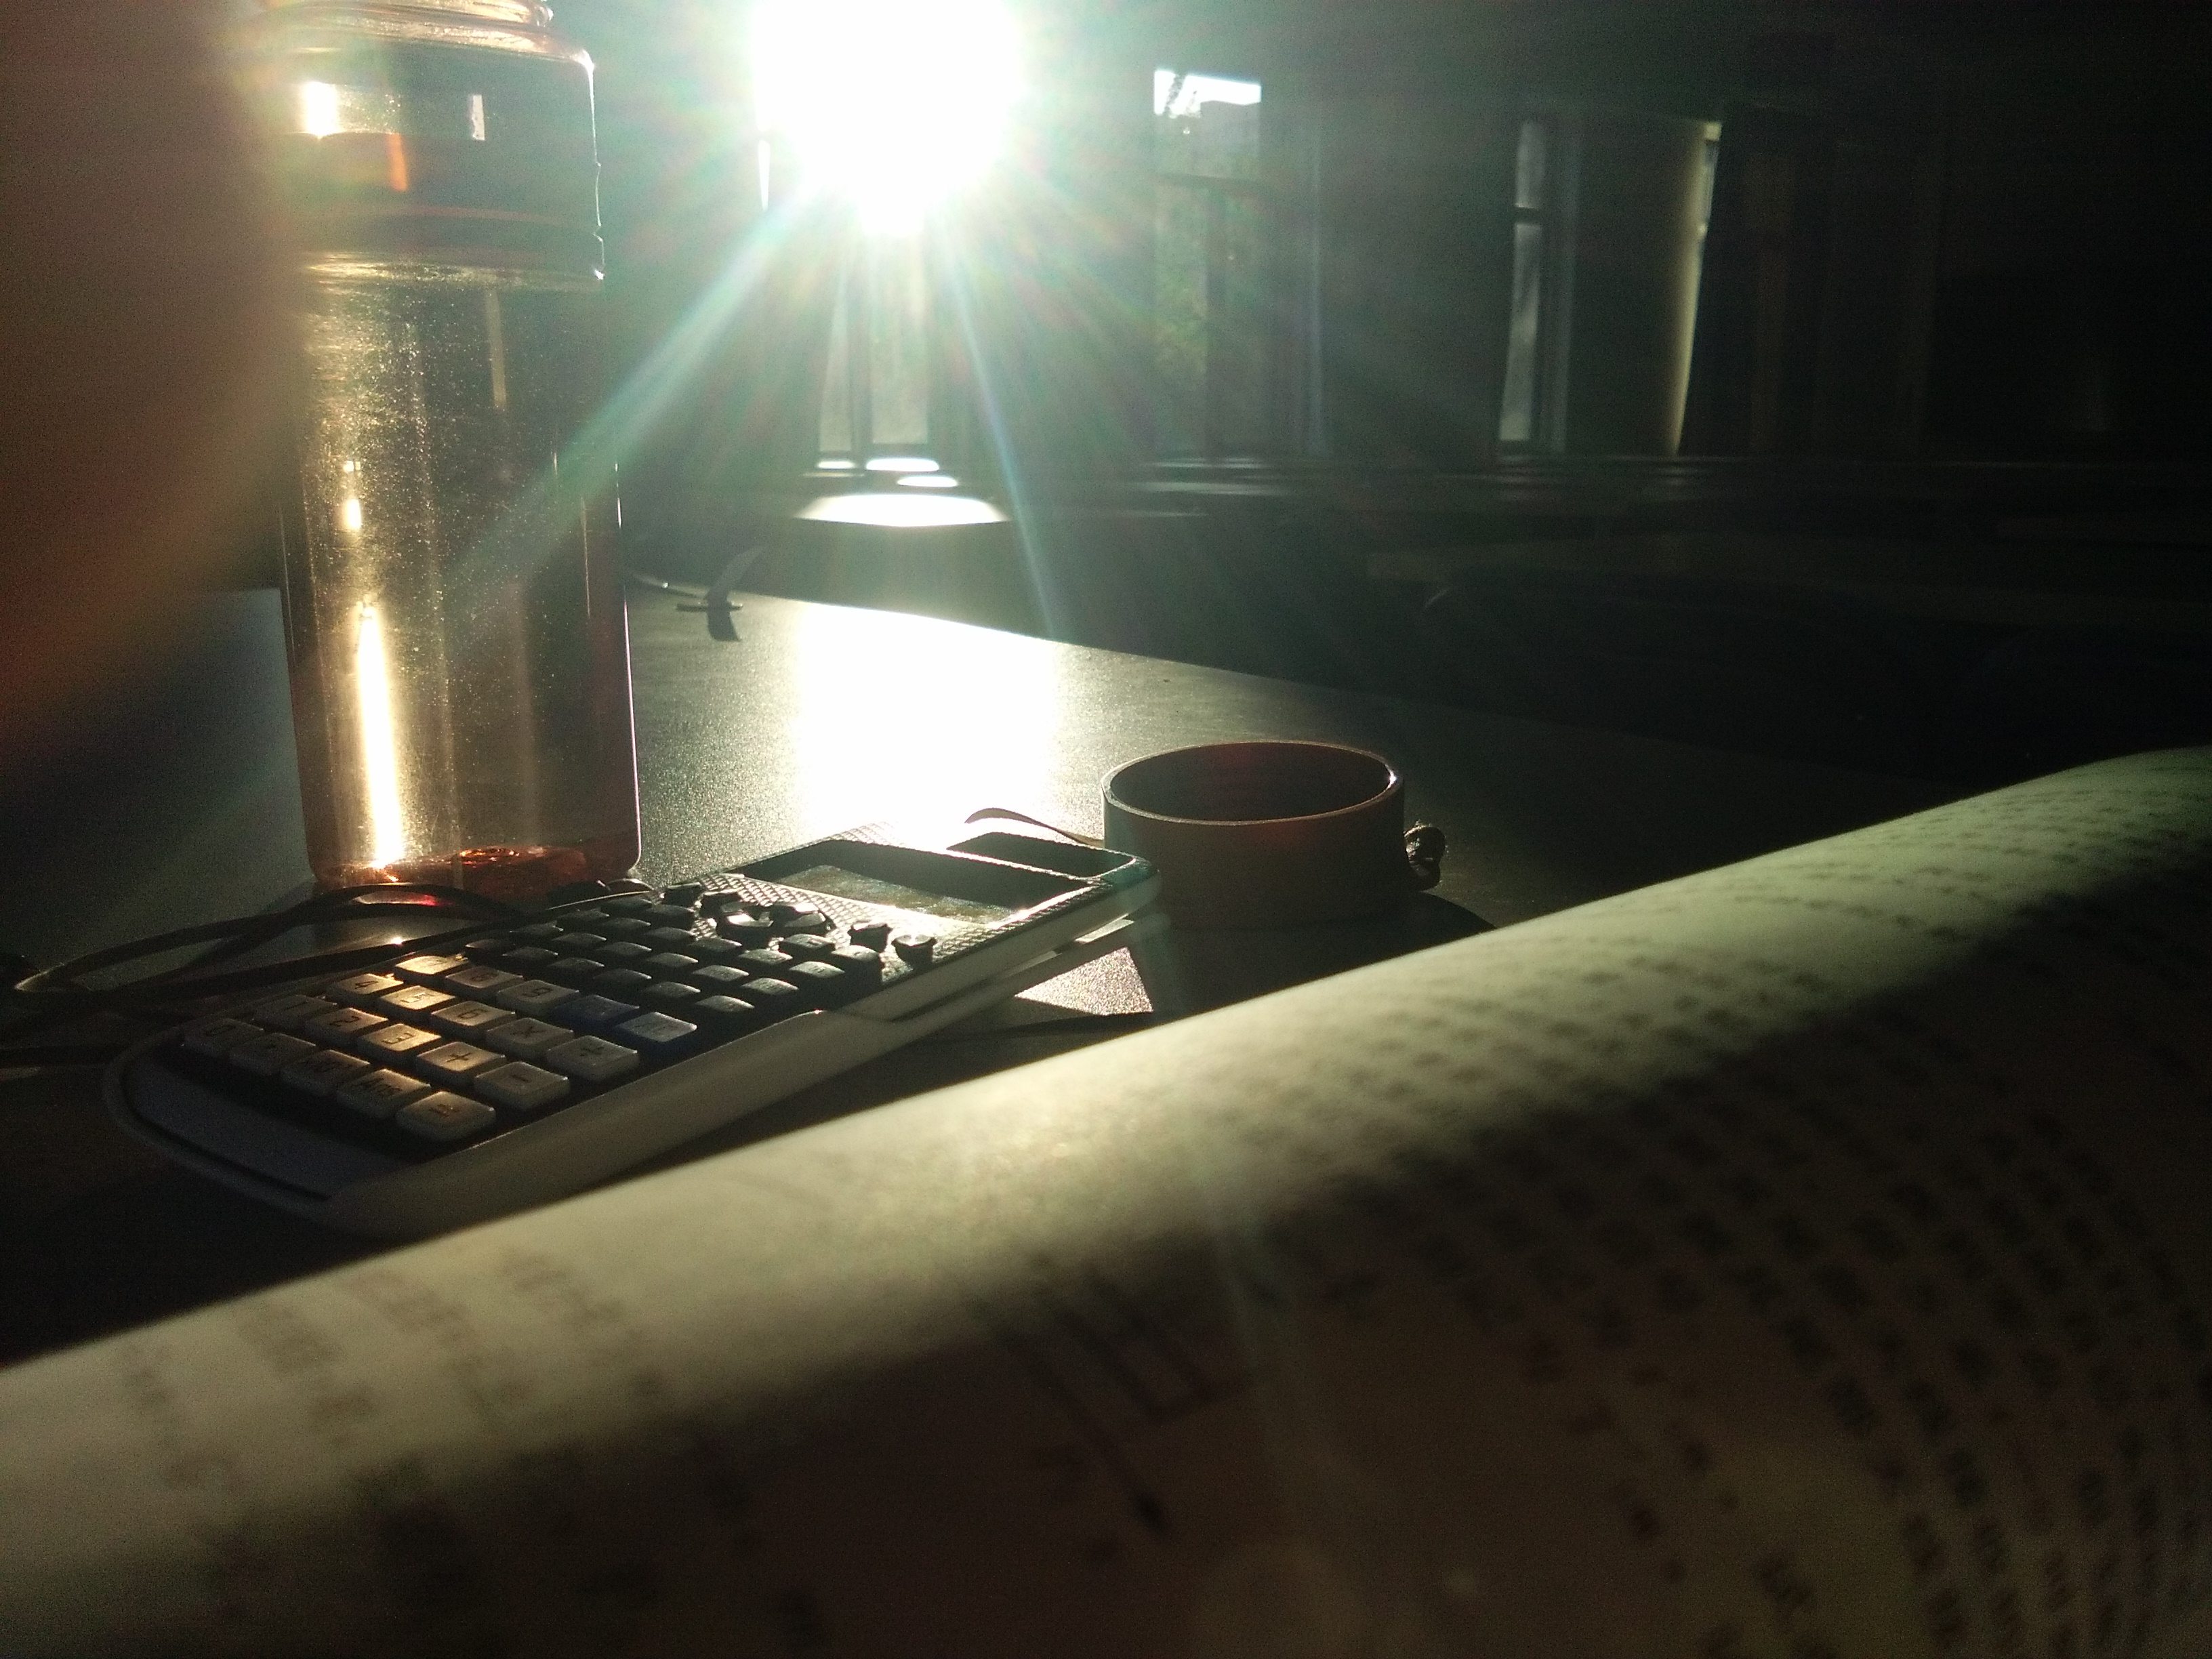
\includegraphics[width=6cm]{IMG_20190520_184311.jpg}
\end{figure}
这段时间我的数理基础也有很大提升,我开始不满足于普通物理,开始学更深入的数学和物理,我对大学物理课程有了一个大致的了解,便开始自学数理方法,线性代数,还有四大力学的部分内容\footnote{数理方法用的是北大吴崇试先生的那本,线性代数国内的书普遍不太好(丘维生先生的除外),于是用了Gilbert的Introduction of Linear Algebra,清华大学出版社;理论力学看了一部分Landau的第一卷,电动力学看了一部分Grimths,还有国内刘觉平老师的书;热统看了一部分林宗涵和Berkeley的物理学教程,量子只看了一些赵凯华老师书上的内容(穿插了一些landau)},还接触了一些微分几何与广义相对论的内容(Landau和梁灿彬)。

停课大概6个月的时间,迎来了36届复赛,刚开始的理论成绩还行,但是也存在时间分配上的问题
\begin{figure}[H]
    \centering
    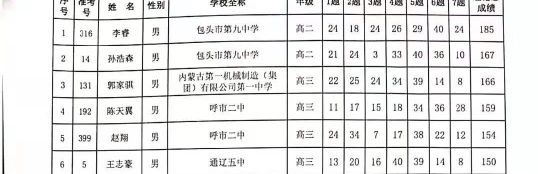
\includegraphics[width=8cm]{qq_pic_merged_1569110757334.jpg}
\end{figure}
在实验时却出了差错
\begin{figure}[H]
    \centering
    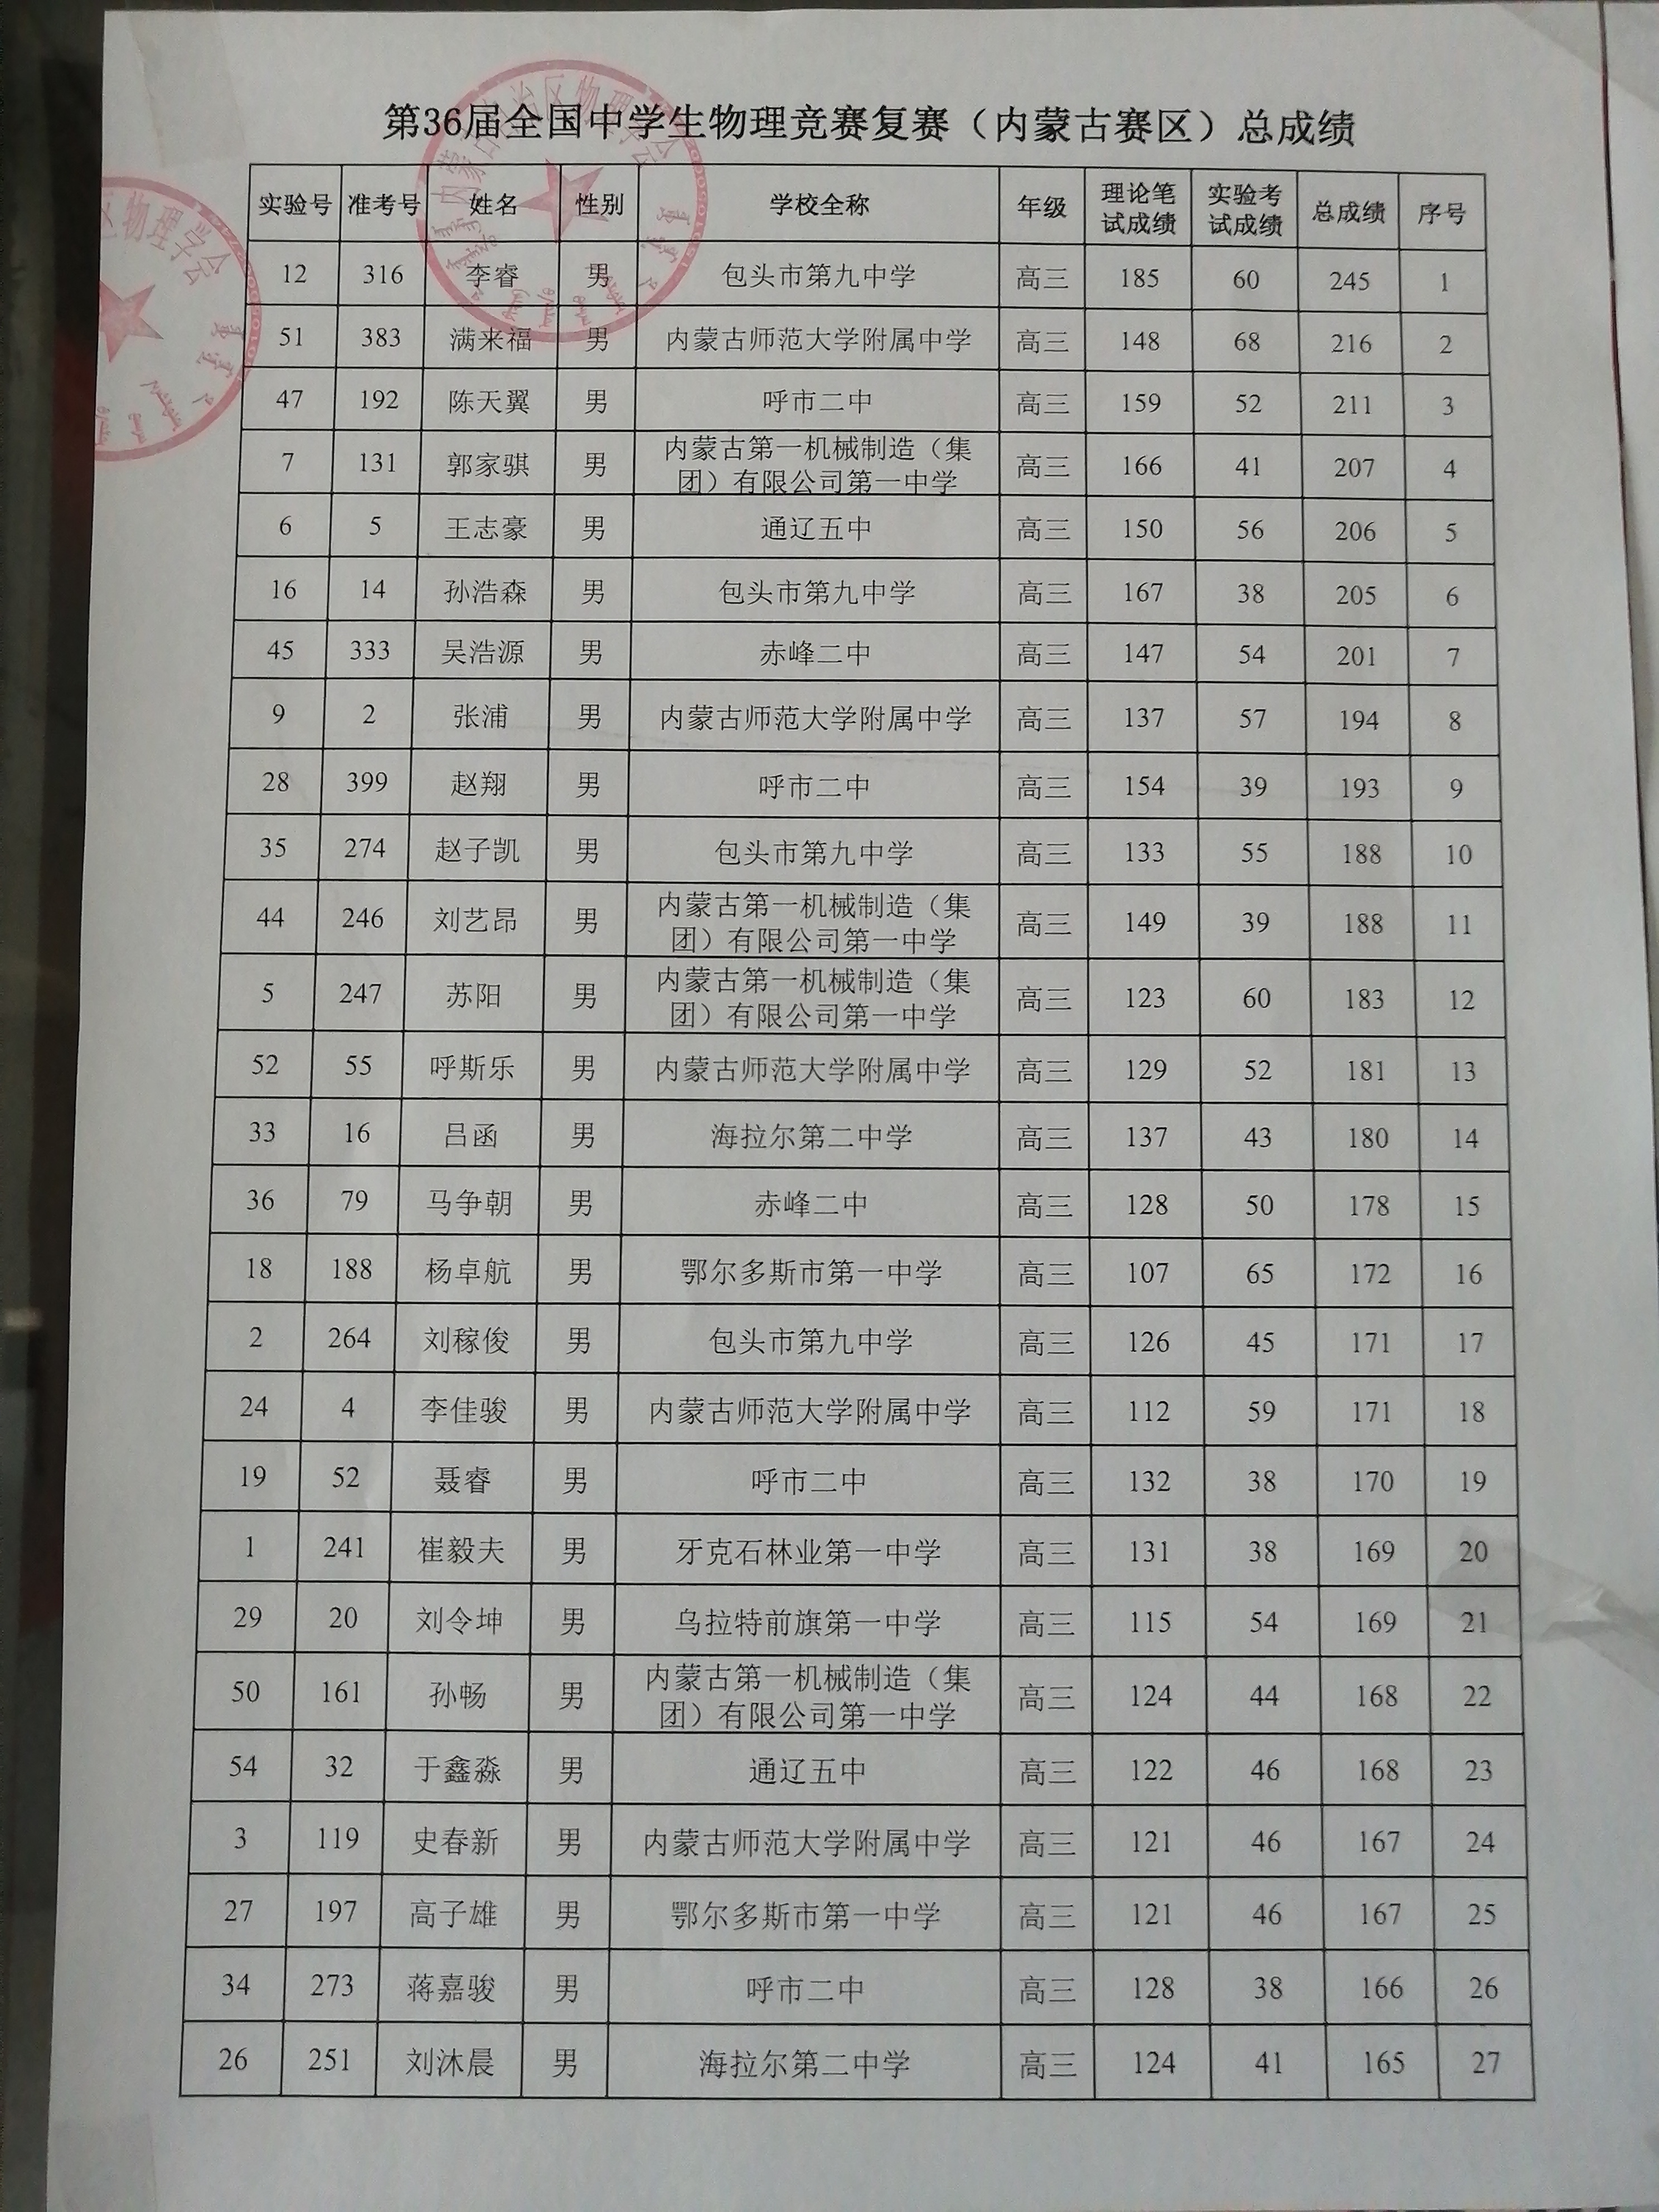
\includegraphics[width=4cm]{IMG20190923090754.jpg}
    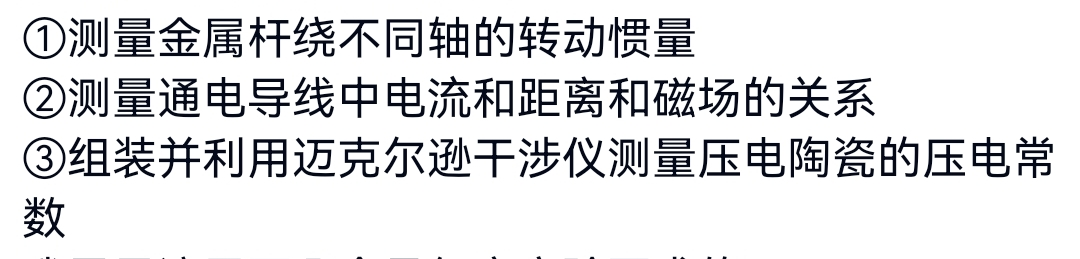
\includegraphics[width=8cm]{Screenshot_20210907_141255.jpg}
\end{figure}
最后无缘决赛,还是有点可惜的

然后就是回归正常高考,虽然中途赶上疫情,居家学习,这期间自学了一些电脑技术,比如你现在看到的这篇文章,就是使用当时学的\LaTeX 语法写的,还做了一些数学物理的科普视频之类的\footnote{\url{https://www.bilibili.com/video/BV1Z7411j7mB}},在贴吧,知乎,超理论坛都有一些科普。自主招生的取消使得省一奖一文不值,高考分数不理想,还有想学物理的愿望,于是来到山西大学

高考后举办了一届百度物理吧的吧赛,出了一些题目
\begin{figure}[H]
    \centering
    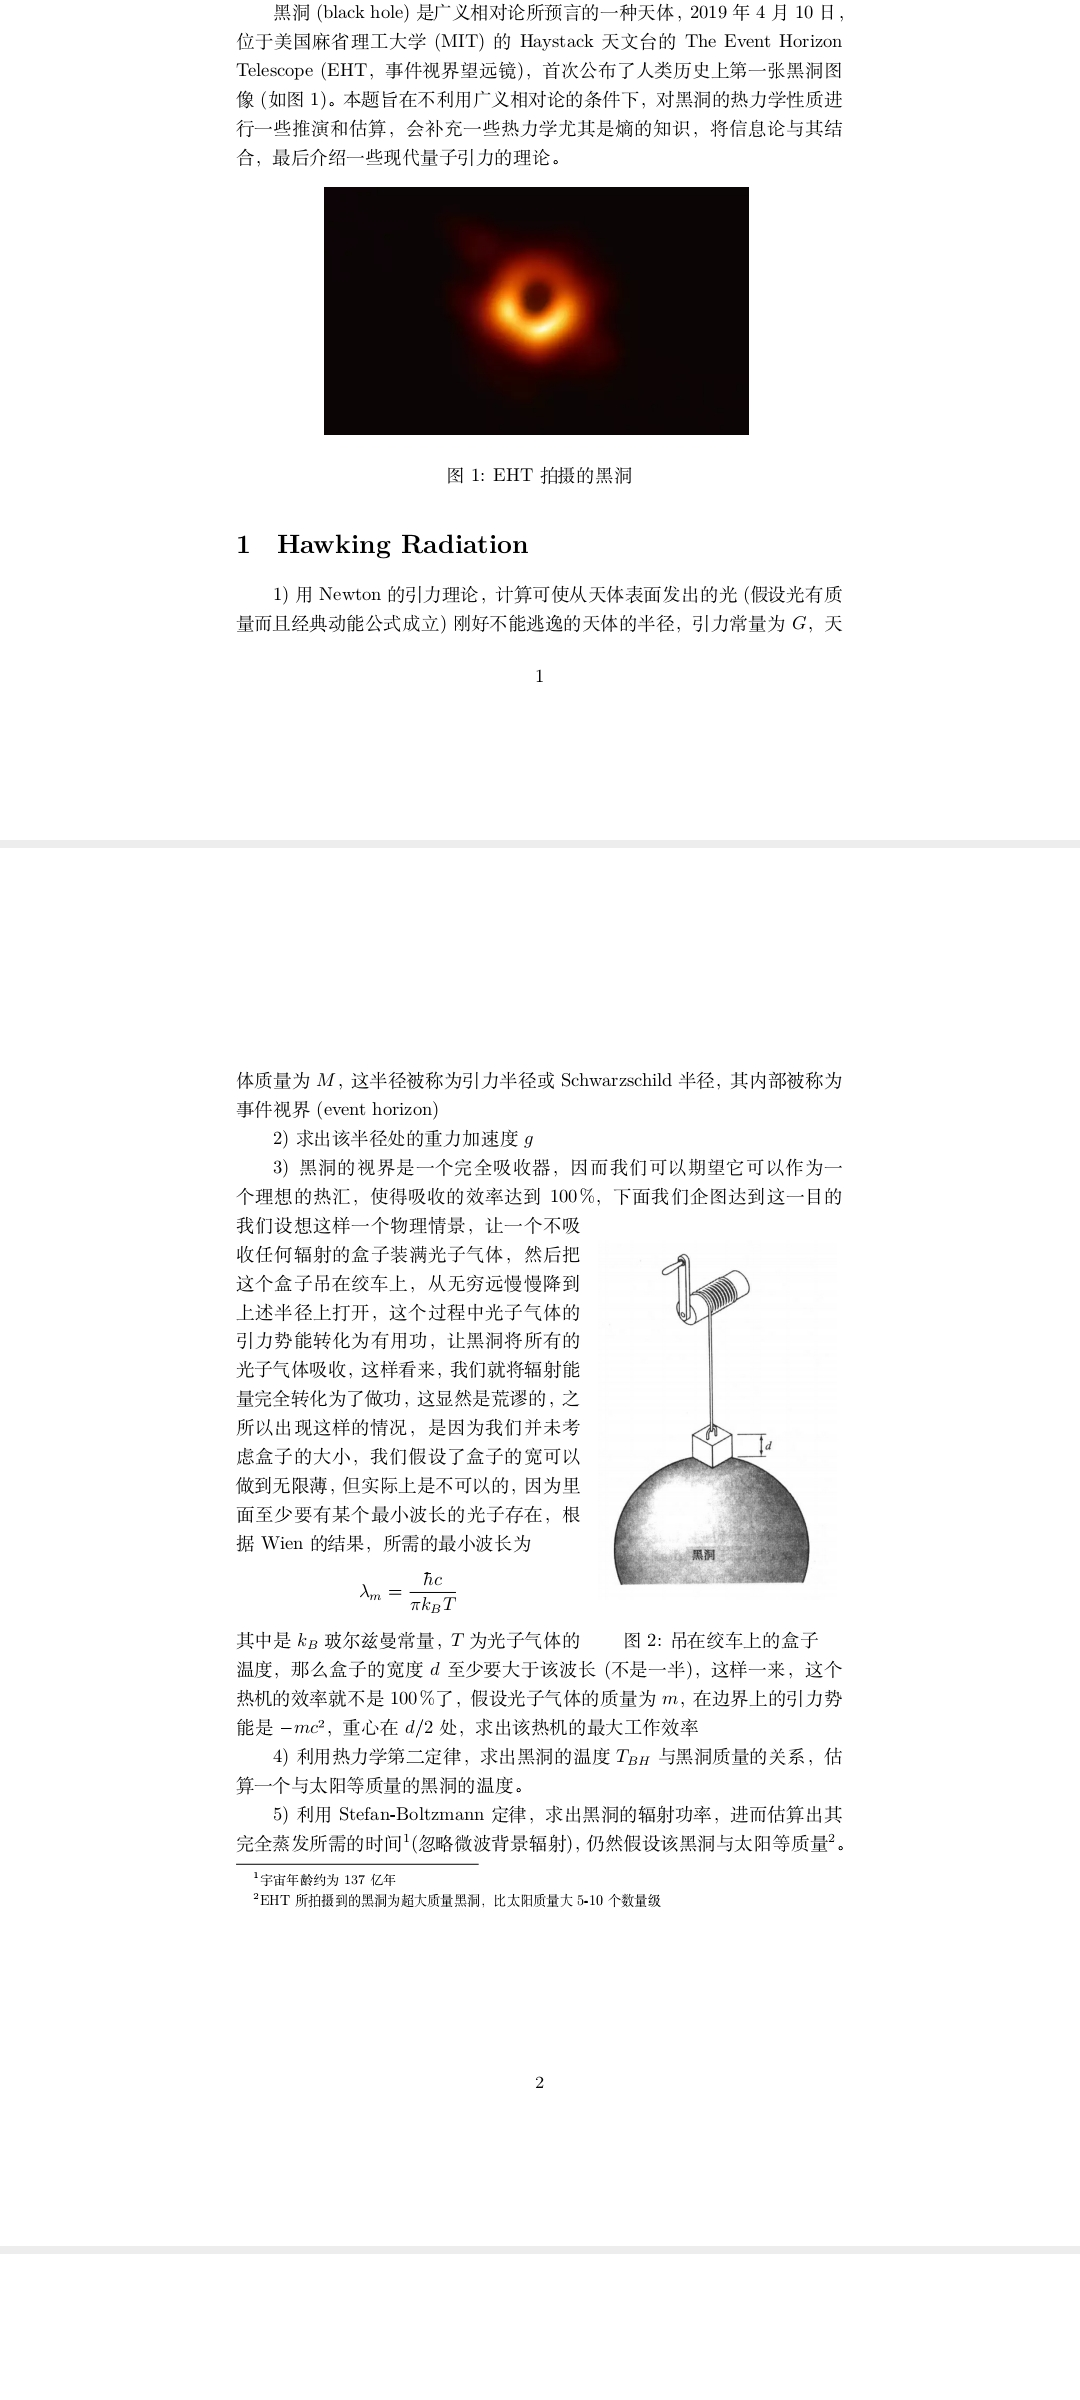
\includegraphics[width=4cm]{Screenshot_20210907_144556_cn.wps.moffice_eng.jpg}
    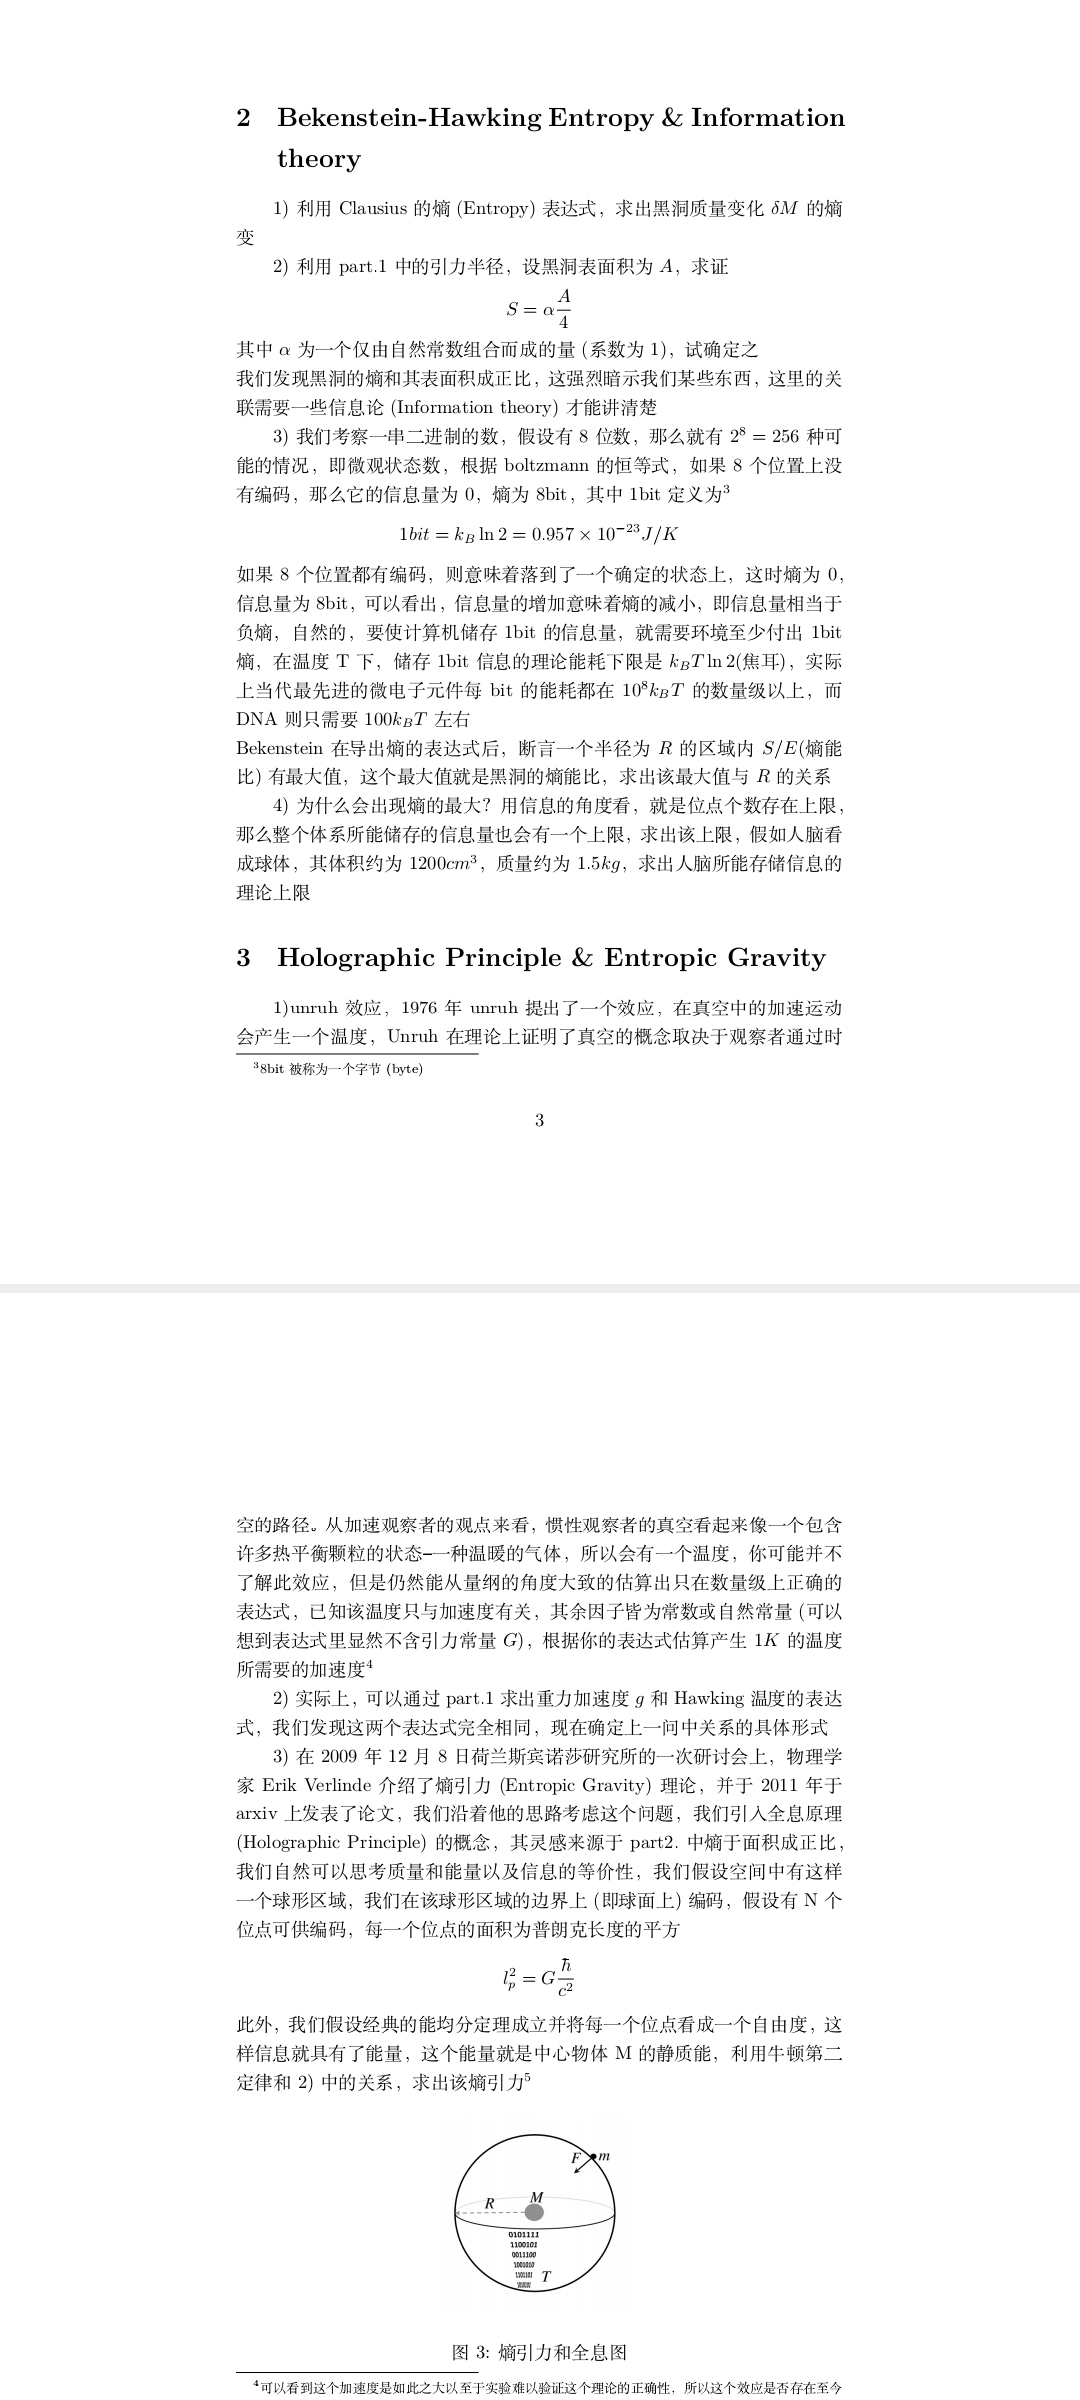
\includegraphics[width=4cm]{Screenshot_20210907_144604_cn.wps.moffice_eng.jpg}
\end{figure}
\section{大学及之后的我自己}
旅游管理是服从调剂的结果,这个专业在大一的课非常少,以至于我可以自己学一些东西,我再一次加固了自己的数理基础,觉得翻译外文书籍是一个比较好的路线,于是开始自己翻译一本数学物理方法的书A Course in Modern Mathematical Physics,Peter Szekeres这本书读来比较对我口味,从集合论讲起,有群论, Hilbert空间和微分几何的内容,
\begin{figure}[H]
    \centering
    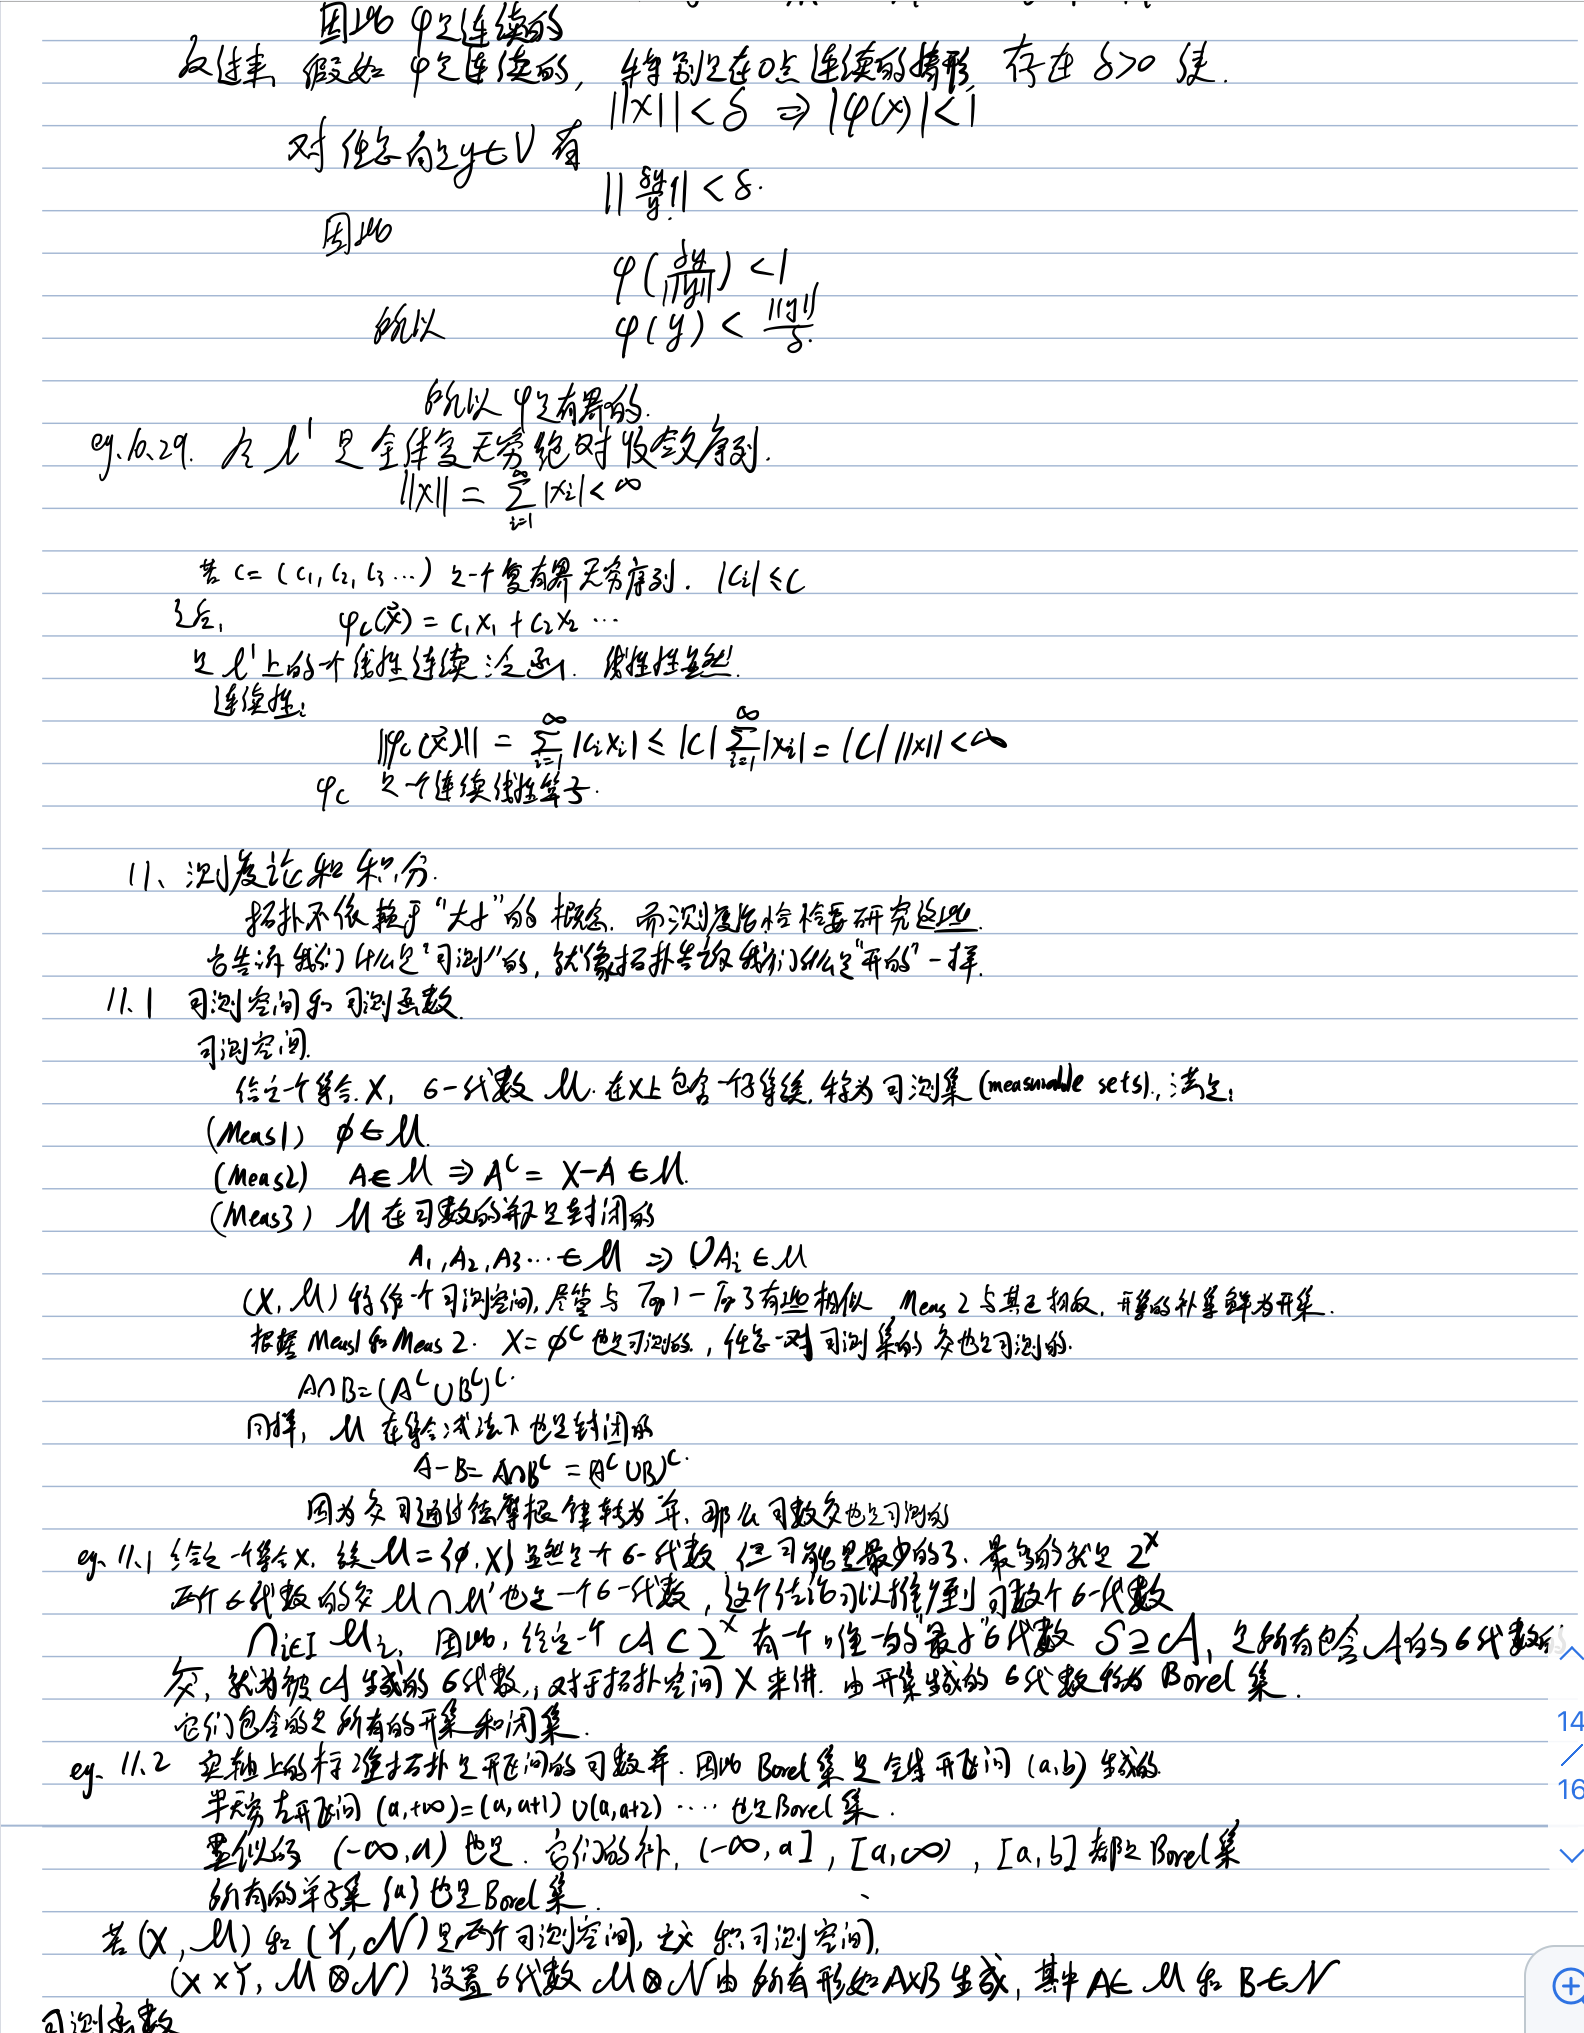
\includegraphics[width=6cm]{690A1E73E094CE8F4FB7D0F57BCEEF22.png}
    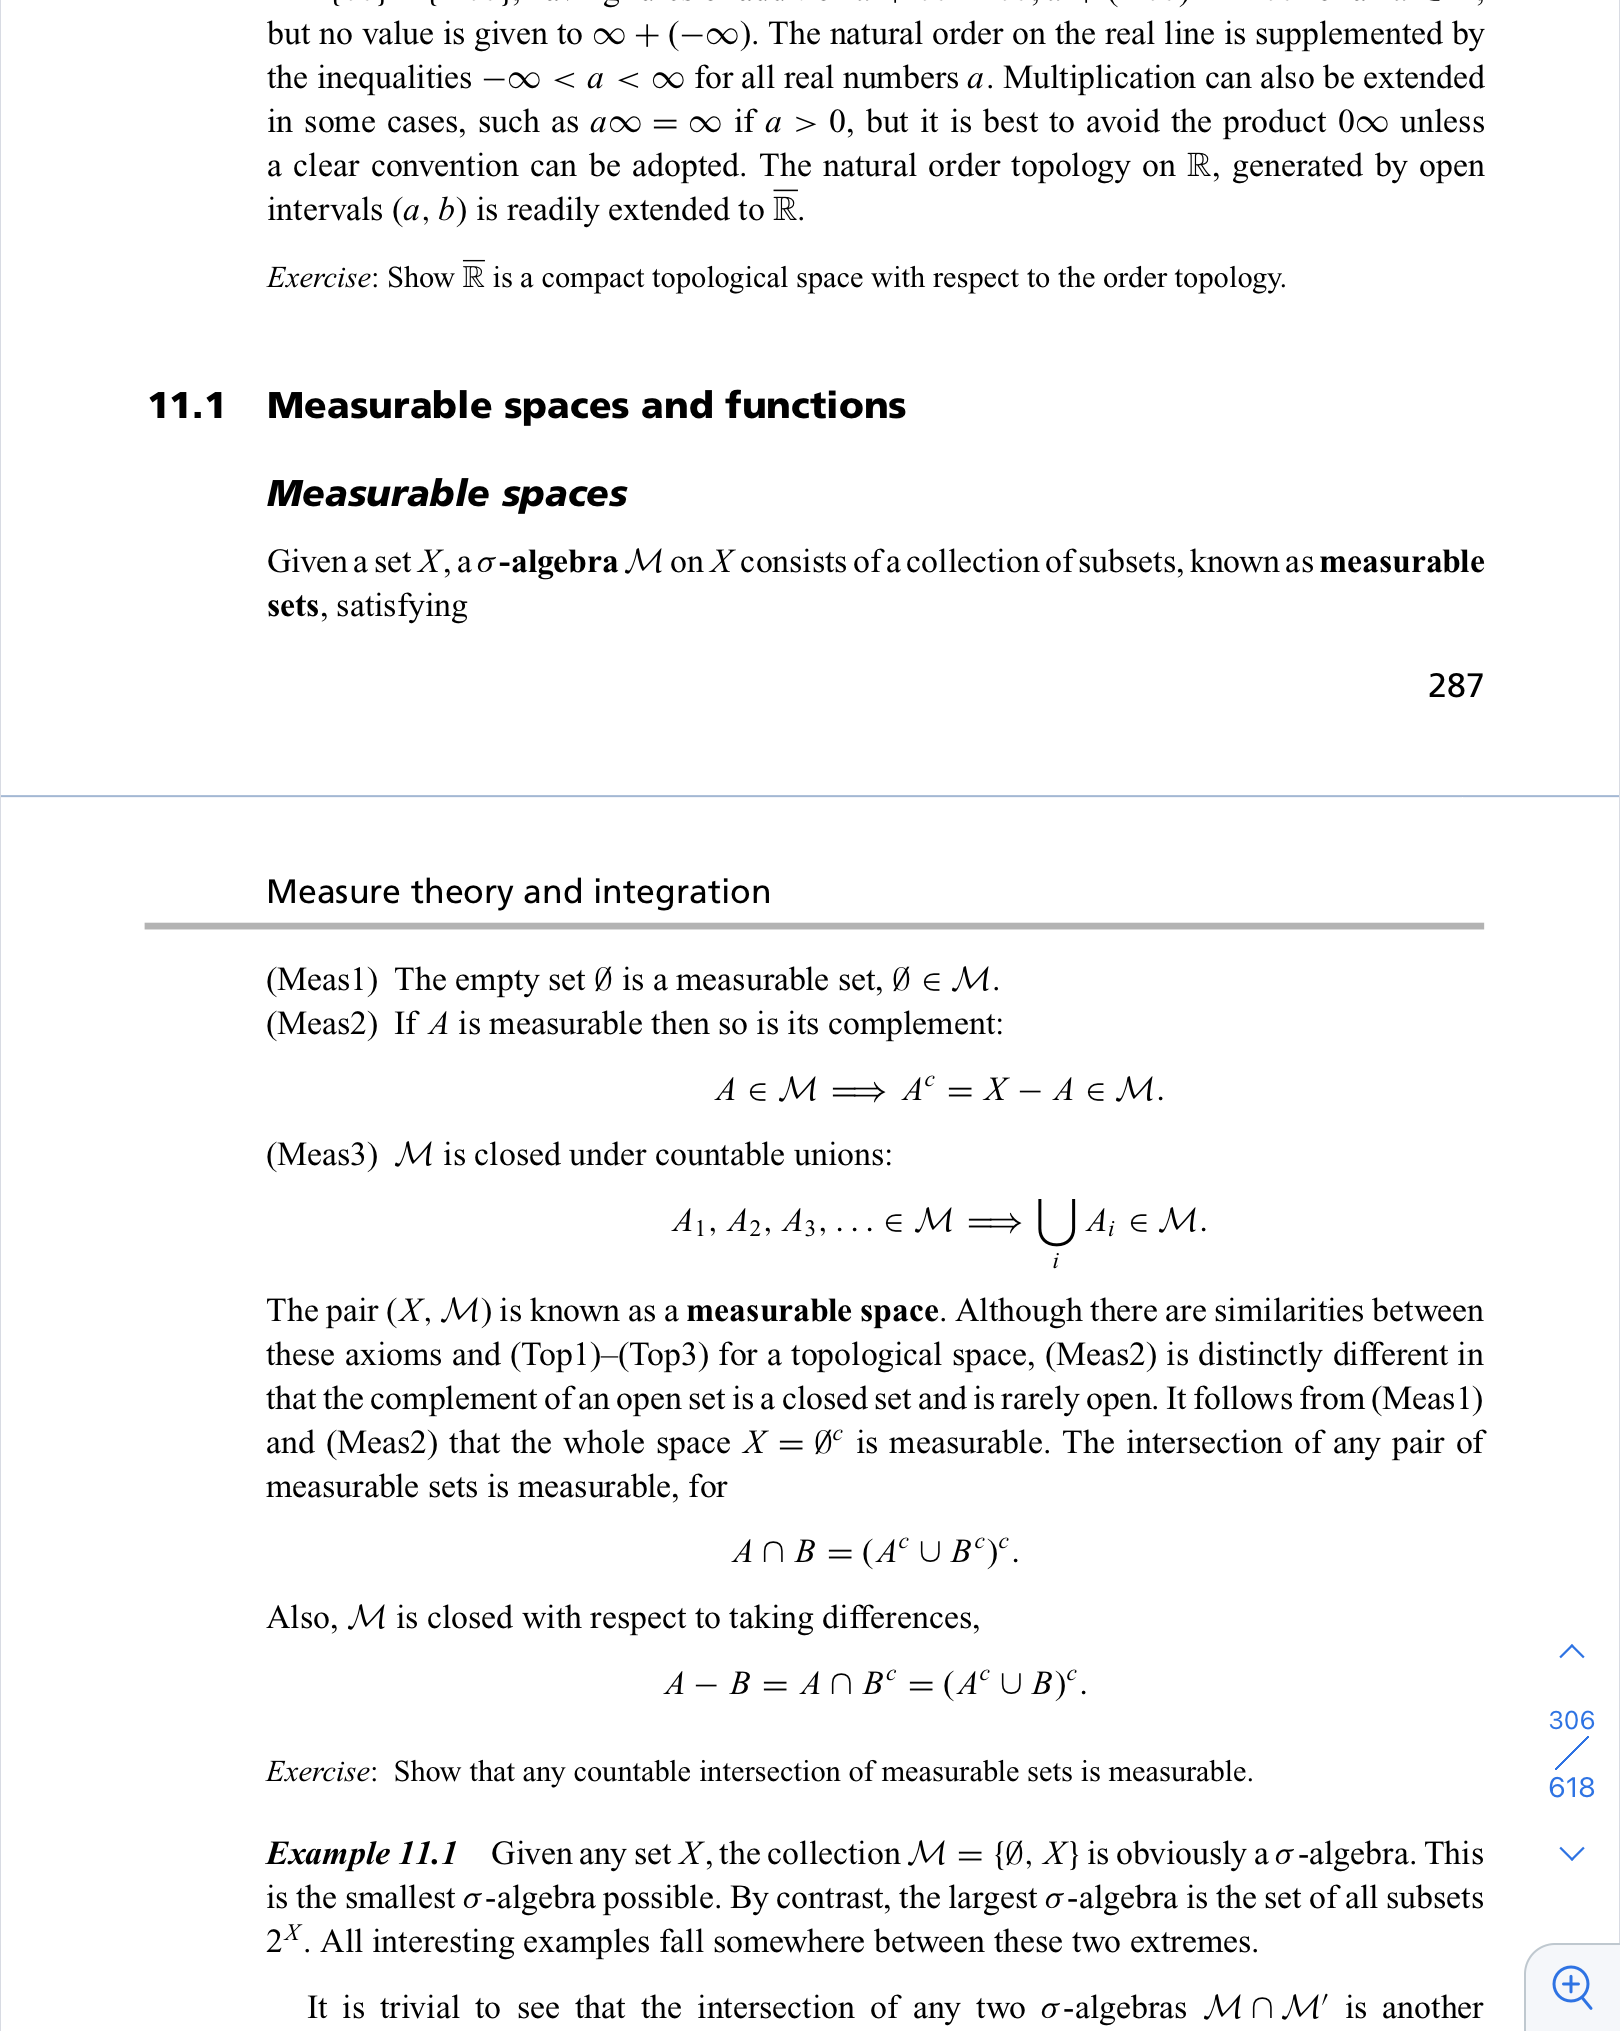
\includegraphics[width=6cm]{9DAFEFAC378DD8114C15D0D3970E29B2.png}
\end{figure}
在旅管的大一也学了一些Python编程和Mathematica编程,会写一些简单的爬虫程序和符号计算的程序,还有精进了自己的\LaTeX 技能,跟从旅管那边的老师做了一些那边的科研训练,关于一些文化遗产的,我负责数据处理和整篇文章的\LaTeX 排版
\begin{figure}[H]
    \centering
    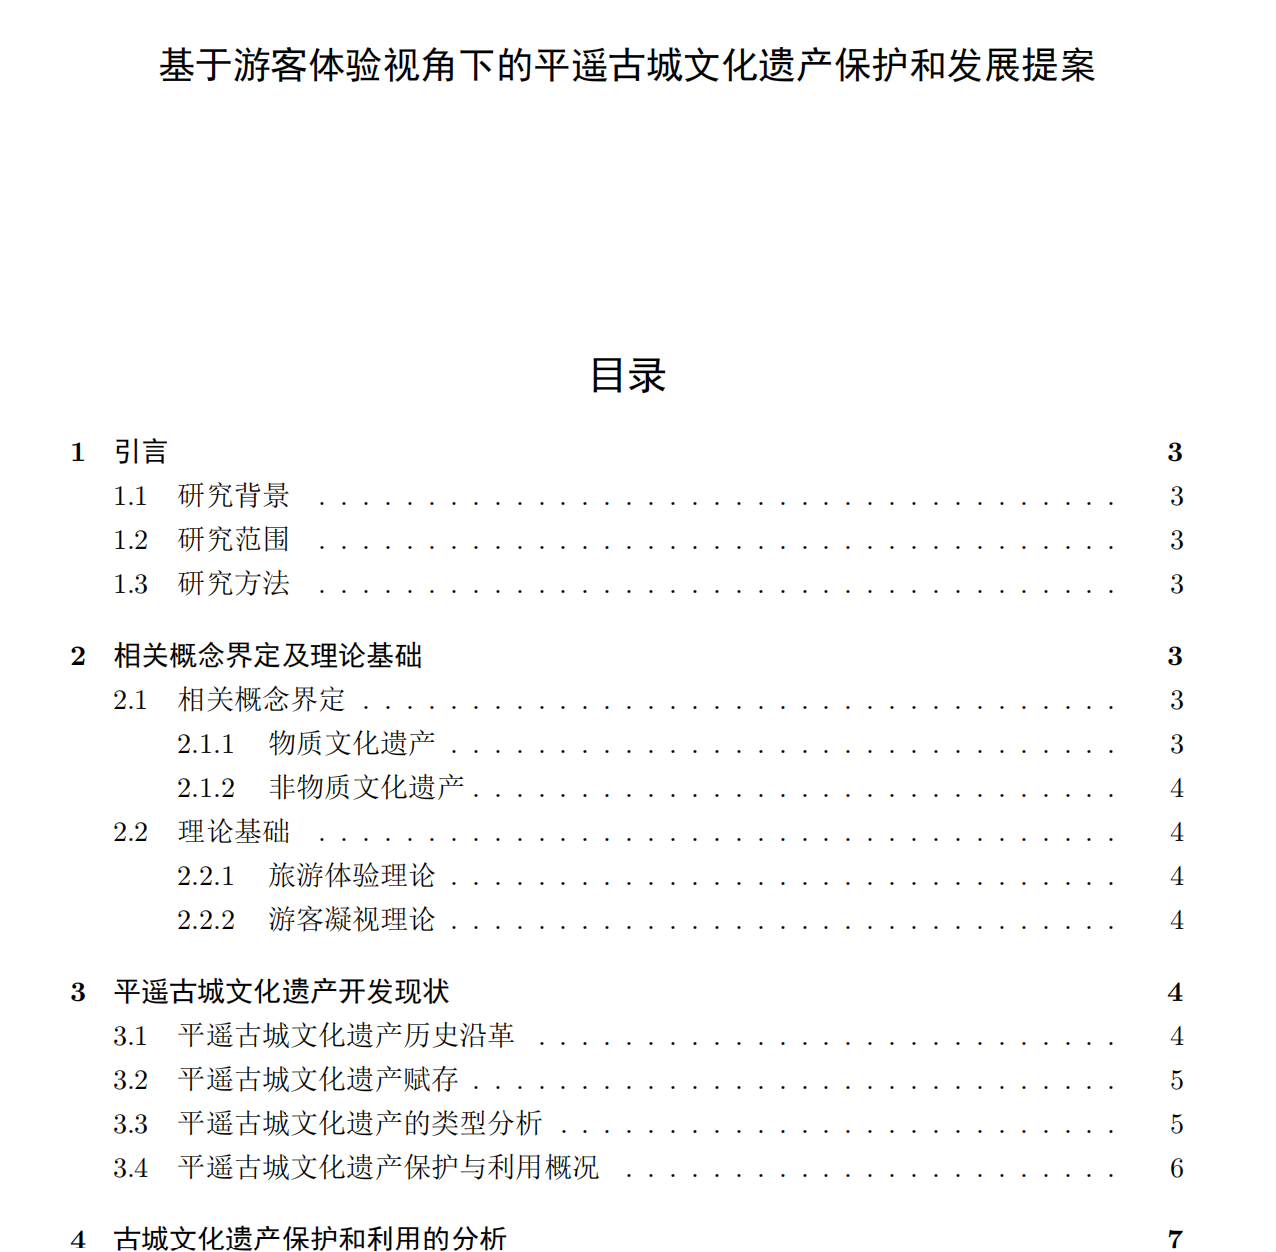
\includegraphics[width=6cm]{屏幕截图 2021-09-07 152214.png}
    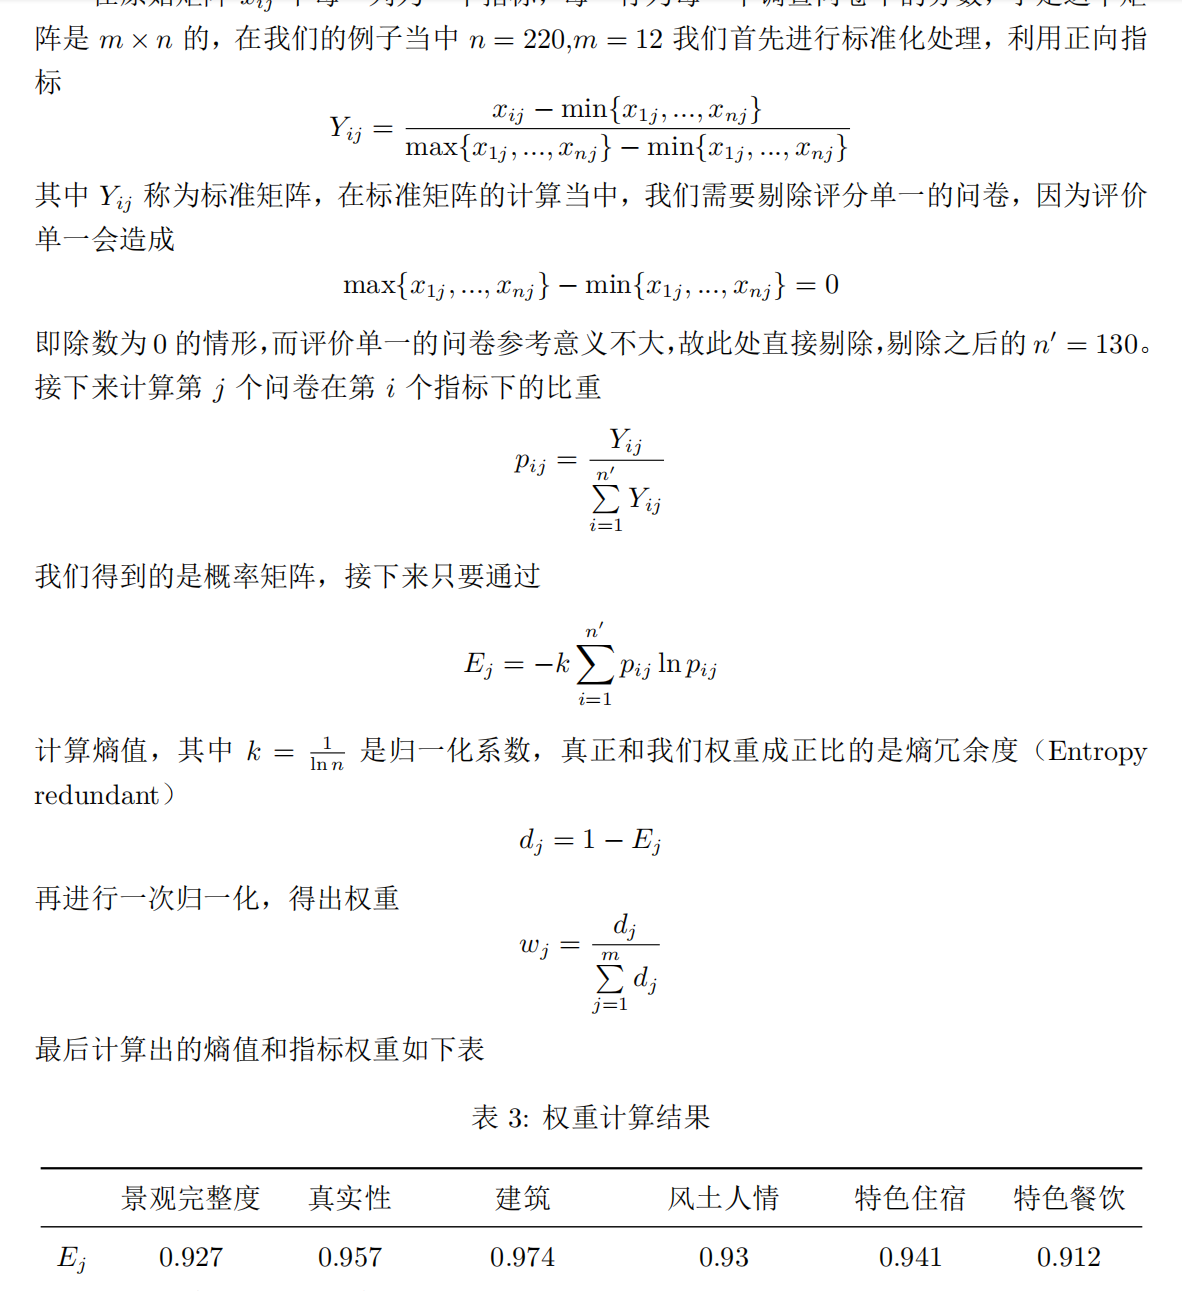
\includegraphics[width=6cm]{屏幕截图 2021-09-07 152300.png}
\end{figure}
英语过了四级,也算是比较圆满吧,没参加数模竞赛有点小遗憾
\part{今后的打算}
学习方面,虽然高中学了很多,但是大学中也不能松懈,而且也没有检测自己学的到底怎么样,来到新专业可以检测一下,我觉得在数学物理的学习中,讨论是极其重要的环节,如果班级有一个良好的讨论氛围,这样大家的学术之风就会正,学习起来也会比较快乐。还有可以把手边还有互联网上的资源利用起来,b站和知乎还有一些小众的论坛上有很多很不错的数学物理课程和文章,网上也有sci-hub等网站可以查找文献。

除了专业课,还有英语要好好学,接下来要尽早过六级,之后雅思托福也要尽快学了

竞赛方面,先打CUPT和数模,大学生数学竞赛或许也可以打一打

编程方面要认真学习C语言和Matlab,Python和Mathematica也要加强

科研方面,我个人是非常希望能在大一期间进入课题组参与组会讨论的,就是不知道有没有机会,还有不知道老师们的研究方向,我个人想做偏理论的方向(可能这个想法比较幼稚)但是我还是想尝试一下,有不会的地方可以学,我觉得我从以往的经历中收获最大的就是学习能力,希望能进组在物电学到更多东西。

班级生活的话,去年大学里除学习之外的事情也蛮多的,不知道物电这边怎么样,总之各类活动就是积极配合团组织和学校,平时生活中也是可以和大家打成一片的。另外我还是天文社团的学术部部长,但也应该不会特别忙

要说的就这么多吧,科研是我一直以来的愿望,我也希望能在物电有新的成长。
\begin{figure}[H]
    \centering
    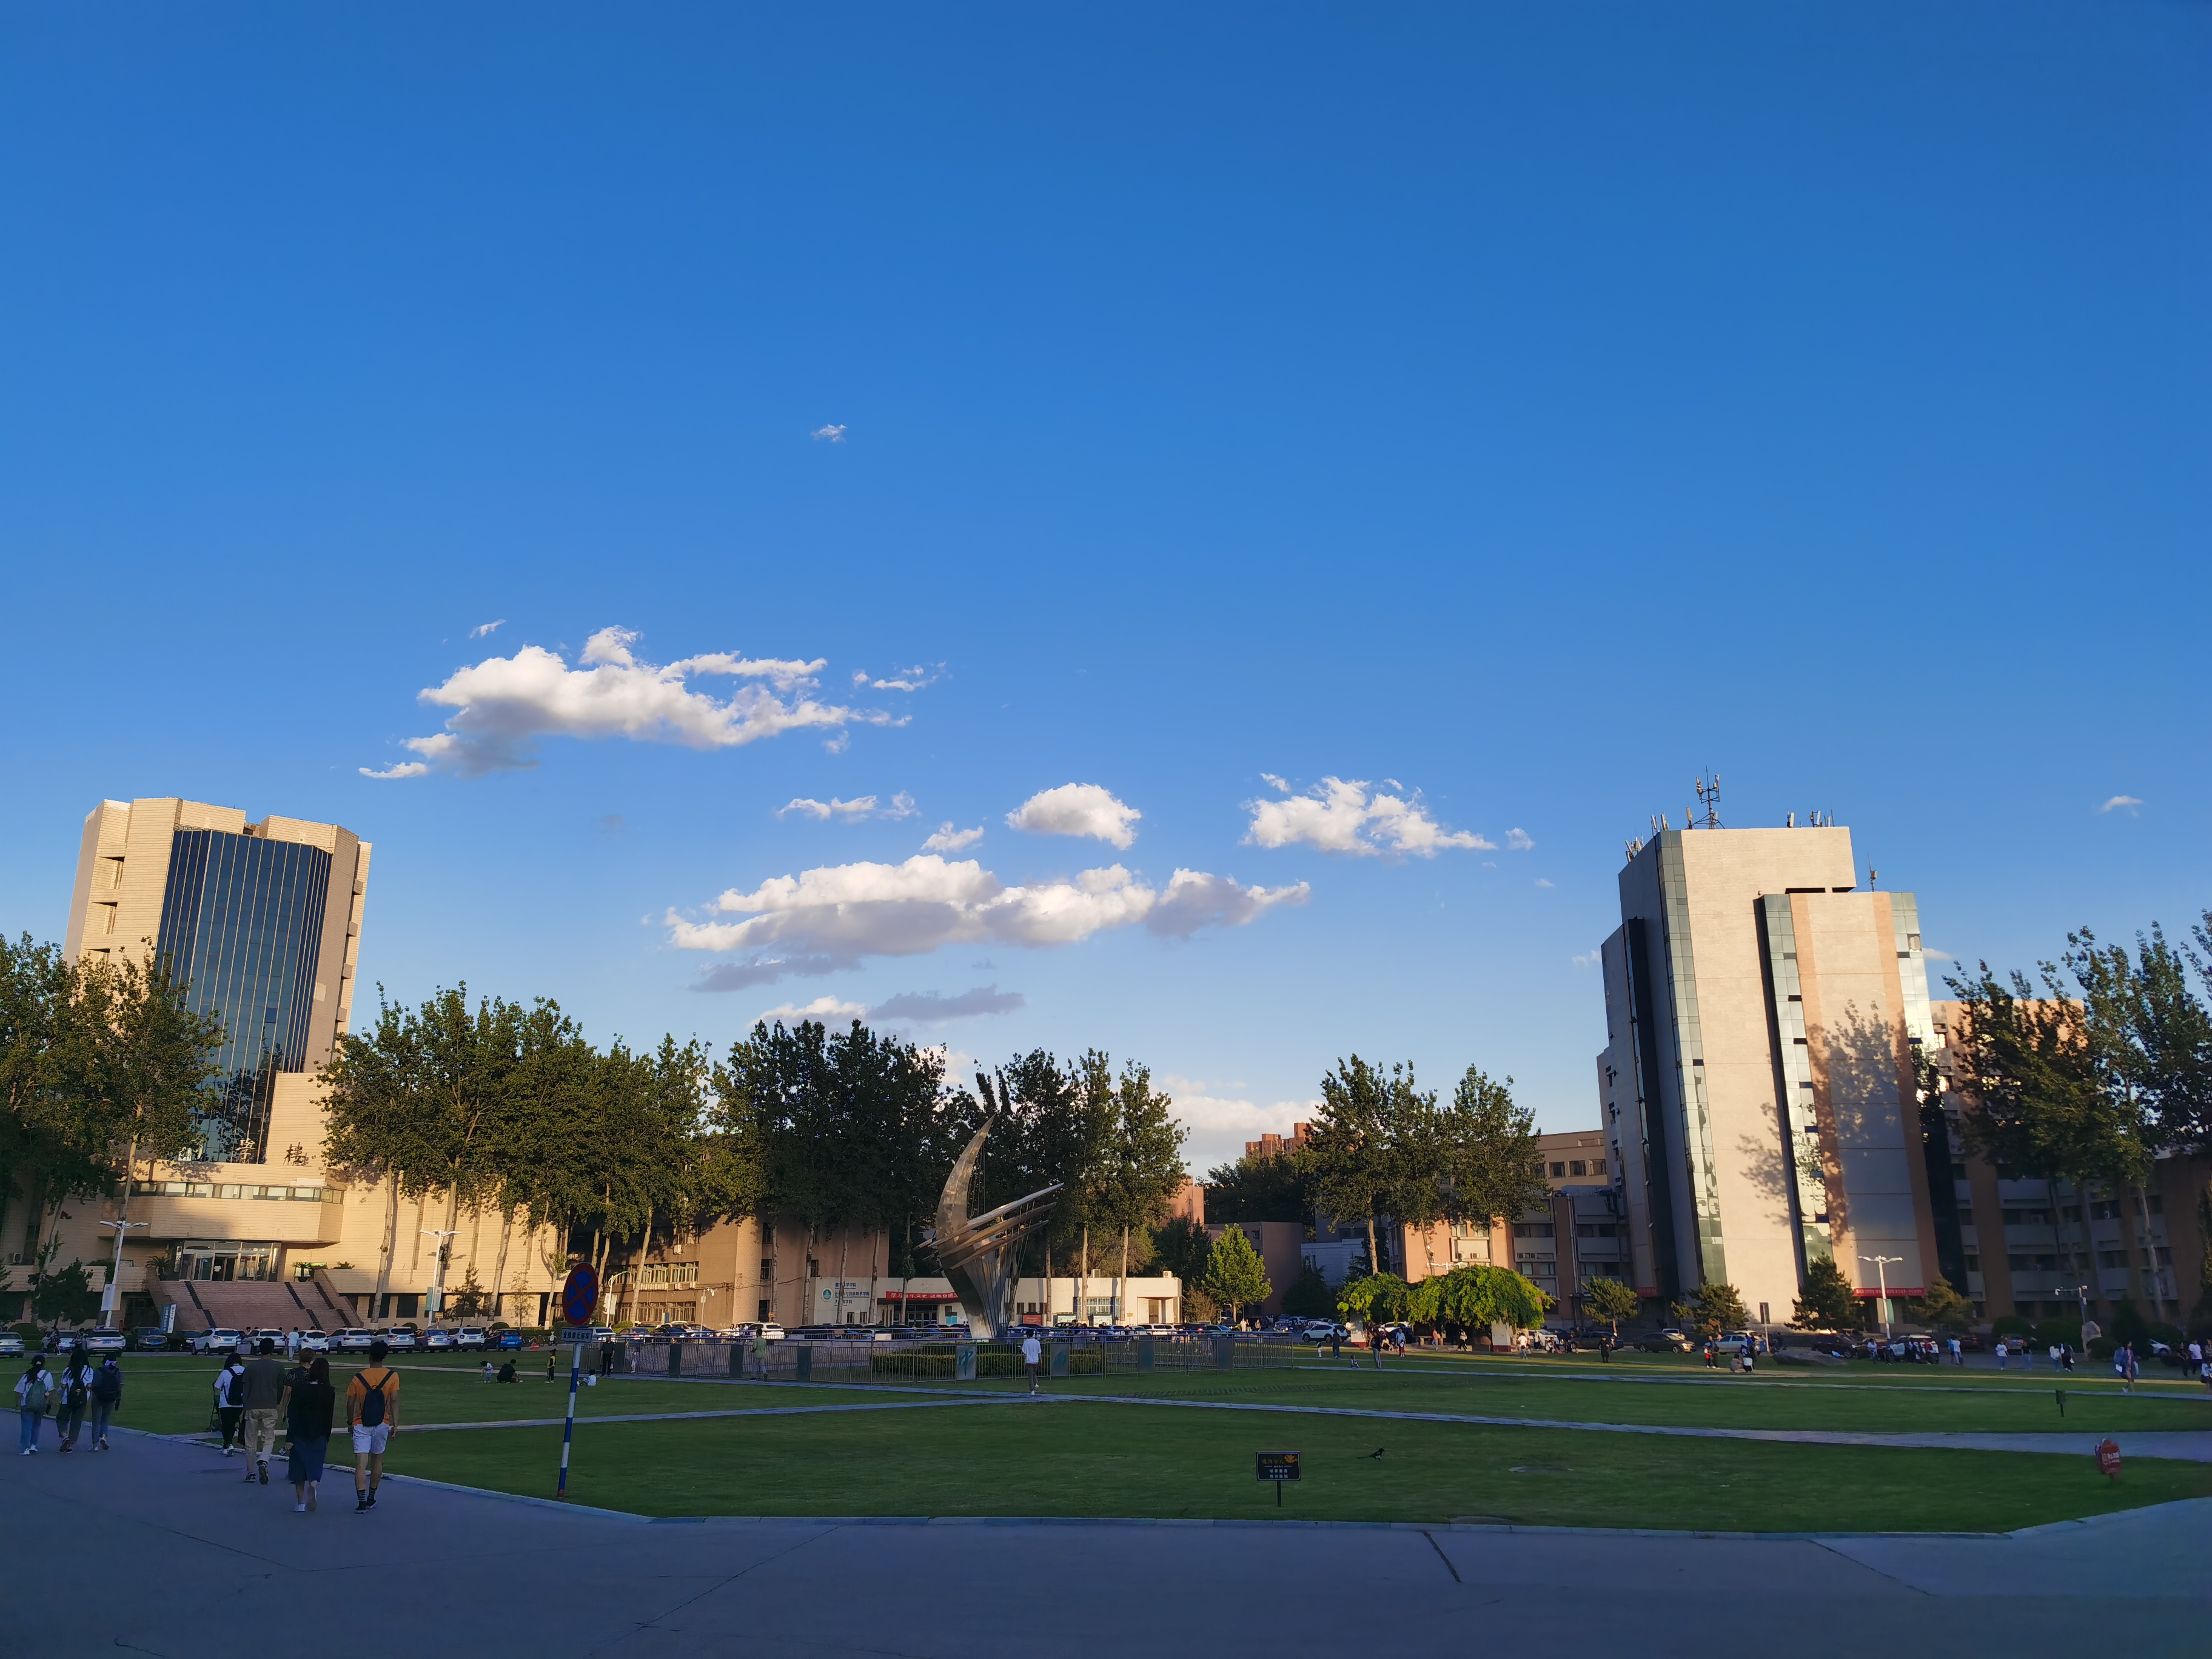
\includegraphics[width=10cm]{IMG_20210526_190810.jpg}
\end{figure}
\end{document}
